
%% bare_jrnl_compsoc.tex
%% V1.4b
%% 2015/08/26
%% by Michael Shell
%% See:
%% http://www.michaelshell.org/
%% for current contact information.
%%
%% This is a skeleton file demonstrating the use of IEEEtran.cls
%% (requires IEEEtran.cls version 1.8b or later) with an IEEE
%% Computer Society journal paper.
%%
%% Support sites:
%% http://www.michaelshell.org/tex/ieeetran/
%% http://www.ctan.org/pkg/ieeetran
%% and
%% http://www.ieee.org/

%%*************************************************************************
%% Legal Notice:
%% This code is offered as-is without any warranty either expressed or
%% implied; without even the implied warranty of MERCHANTABILITY or
%% FITNESS FOR A PARTICULAR PURPOSE! 
%% User assumes all risk.
%% In no event shall the IEEE or any contributor to this code be liable for
%% any damages or losses, including, but not limited to, incidental,
%% consequential, or any other damages, resulting from the use or misuse
%% of any information contained here.
%%
%% All comments are the opinions of their respective authors and are not
%% necessarily endorsed by the IEEE.
%%
%% This work is distributed under the LaTeX Project Public License (LPPL)
%% ( http://www.latex-project.org/ ) version 1.3, and may be freely used,
%% distributed and modified. A copy of the LPPL, version 1.3, is included
%% in the base LaTeX documentation of all distributions of LaTeX released
%% 2003/12/01 or later.
%% Retain all contribution notices and credits.
%% ** Modified files should be clearly indicated as such, including  **
%% ** renaming them and changing author support contact information. **
%%*************************************************************************


% *** Authors should verify (and, if needed, correct) their LaTeX system  ***
% *** with the testflow diagnostic prior to trusting their LaTeX platform ***
% *** with production work. The IEEE's font choices and paper sizes can   ***
% *** trigger bugs that do not appear when using other class files.       ***                          ***
% The testflow support page is at:
% http://www.michaelshell.org/tex/testflow/


\documentclass[10pt,journal,compsoc]{IEEEtran}
%
% If IEEEtran.cls has not been installed into the LaTeX system files,
% manually specify the path to it like:
% \documentclass[10pt,journal,compsoc]{../sty/IEEEtran}

\usepackage{graphicx}
\usepackage{algpseudocode}
\usepackage{subfigure}
\usepackage{tabularx,booktabs}
\usepackage{amssymb,amsfonts,amsthm,amsmath}
\usepackage{textcomp}
\usepackage{xcolor}
\usepackage{url}
\usepackage{multirow}
\usepackage{pifont}
\usepackage[nocompress]{cite}
\usepackage[linesnumbered,ruled]{algorithm2e}

% Some very useful LaTeX packages include:
% (uncomment the ones you want to load)


% *** MISC UTILITY PACKAGES ***
%
%\usepackage{ifpdf}
% Heiko Oberdiek's ifpdf.sty is very useful if you need conditional
% compilation based on whether the output is pdf or dvi.
% usage:
% \ifpdf
%   % pdf code
% \else
%   % dvi code
% \fi
% The latest version of ifpdf.sty can be obtained from:
% http://www.ctan.org/pkg/ifpdf
% Also, note that IEEEtran.cls V1.7 and later provides a builtin
% \ifCLASSINFOpdf conditional that works the same way.
% When switching from latex to pdflatex and vice-versa, the compiler may
% have to be run twice to clear warning/error messages.






% *** CITATION PACKAGES ***
%
%\ifCLASSOPTIONcompsoc
%  % IEEE Computer Society needs nocompress option
%  % requires cite.sty v4.0 or later (November 2003)
%  \usepackage[nocompress]{cite}
%\else
%  % normal IEEE
%  \usepackage{cite}
%\fi
% cite.sty was written by Donald Arseneau
% V1.6 and later of IEEEtran pre-defines the format of the cite.sty package
% \cite{} output to follow that of the IEEE. Loading the cite package will
% result in citation numbers being automatically sorted and properly
% "compressed/ranged". e.g., [1], [9], [2], [7], [5], [6] without using
% cite.sty will become [1], [2], [5]--[7], [9] using cite.sty. cite.sty's
% \cite will automatically add leading space, if needed. Use cite.sty's
% noadjust option (cite.sty V3.8 and later) if you want to turn this off
% such as if a citation ever needs to be enclosed in parenthesis.
% cite.sty is already installed on most LaTeX systems. Be sure and use
% version 5.0 (2009-03-20) and later if using hyperref.sty.
% The latest version can be obtained at:
% http://www.ctan.org/pkg/cite
% The documentation is contained in the cite.sty file itself.
%
% Note that some packages require special options to format as the Computer
% Society requires. In particular, Computer Society  papers do not use
% compressed citation ranges as is done in typical IEEE papers
% (e.g., [1]-[4]). Instead, they list every citation separately in order
% (e.g., [1], [2], [3], [4]). To get the latter we need to load the cite
% package with the nocompress option which is supported by cite.sty v4.0
% and later. Note also the use of a CLASSOPTION conditional provided by
% IEEEtran.cls V1.7 and later.





% *** GRAPHICS RELATED PACKAGES ***
%
\ifCLASSINFOpdf
  % \usepackage[pdftex]{graphicx}
  % declare the path(s) where your graphic files are
  % \graphicspath{{../pdf/}{../jpeg/}}
  % and their extensions so you won't have to specify these with
  % every instance of \includegraphics
  % \DeclareGraphicsExtensions{.pdf,.jpeg,.png}
\else
  % or other class option (dvipsone, dvipdf, if not using dvips). graphicx
  % will default to the driver specified in the system graphics.cfg if no
  % driver is specified.
  % \usepackage[dvips]{graphicx}
  % declare the path(s) where your graphic files are
  % \graphicspath{{../eps/}}
  % and their extensions so you won't have to specify these with
  % every instance of \includegraphics
  % \DeclareGraphicsExtensions{.eps}
\fi
% graphicx was written by David Carlisle and Sebastian Rahtz. It is
% required if you want graphics, photos, etc. graphicx.sty is already
% installed on most LaTeX systems. The latest version and documentation
% can be obtained at: 
% http://www.ctan.org/pkg/graphicx
% Another good source of documentation is "Using Imported Graphics in
% LaTeX2e" by Keith Reckdahl which can be found at:
% http://www.ctan.org/pkg/epslatex
%
% latex, and pdflatex in dvi mode, support graphics in encapsulated
% postscript (.eps) format. pdflatex in pdf mode supports graphics
% in .pdf, .jpeg, .png and .mps (metapost) formats. Users should ensure
% that all non-photo figures use a vector format (.eps, .pdf, .mps) and
% not a bitmapped formats (.jpeg, .png). The IEEE frowns on bitmapped formats
% which can result in "jaggedy"/blurry rendering of lines and letters as
% well as large increases in file sizes.
%
% You can find documentation about the pdfTeX application at:
% http://www.tug.org/applications/pdftex






% *** MATH PACKAGES ***
%
%\usepackage{amsmath}
% A popular package from the American Mathematical Society that provides
% many useful and powerful commands for dealing with mathematics.
%
% Note that the amsmath package sets \interdisplaylinepenalty to 10000
% thus preventing page breaks from occurring within multiline equations. Use:
%\interdisplaylinepenalty=2500
% after loading amsmath to restore such page breaks as IEEEtran.cls normally
% does. amsmath.sty is already installed on most LaTeX systems. The latest
% version and documentation can be obtained at:
% http://www.ctan.org/pkg/amsmath





% *** SPECIALIZED LIST PACKAGES ***
%
%\usepackage{algorithmic}
% algorithmic.sty was written by Peter Williams and Rogerio Brito.
% This package provides an algorithmic environment fo describing algorithms.
% You can use the algorithmic environment in-text or within a figure
% environment to provide for a floating algorithm. Do NOT use the algorithm
% floating environment provided by algorithm.sty (by the same authors) or
% algorithm2e.sty (by Christophe Fiorio) as the IEEE does not use dedicated
% algorithm float types and packages that provide these will not provide
% correct IEEE style captions. The latest version and documentation of
% algorithmic.sty can be obtained at:
% http://www.ctan.org/pkg/algorithms
% Also of interest may be the (relatively newer and more customizable)
% algorithmicx.sty package by Szasz Janos:
% http://www.ctan.org/pkg/algorithmicx




% *** ALIGNMENT PACKAGES ***
%
%\usepackage{array}
% Frank Mittelbach's and David Carlisle's array.sty patches and improves
% the standard LaTeX2e array and tabular environments to provide better
% appearance and additional user controls. As the default LaTeX2e table
% generation code is lacking to the point of almost being broken with
% respect to the quality of the end results, all users are strongly
% advised to use an enhanced (at the very least that provided by array.sty)
% set of table tools. array.sty is already installed on most systems. The
% latest version and documentation can be obtained at:
% http://www.ctan.org/pkg/array


% IEEEtran contains the IEEEeqnarray family of commands that can be used to
% generate multiline equations as well as matrices, tables, etc., of high
% quality.




% *** SUBFIGURE PACKAGES ***
%\ifCLASSOPTIONcompsoc
%  \usepackage[caption=false,font=footnotesize,labelfont=sf,textfont=sf]{subfig}
%\else
%  \usepackage[caption=false,font=footnotesize]{subfig}
%\fi
% subfig.sty, written by Steven Douglas Cochran, is the modern replacement
% for subfigure.sty, the latter of which is no longer maintained and is
% incompatible with some LaTeX packages including fixltx2e. However,
% subfig.sty requires and automatically loads Axel Sommerfeldt's caption.sty
% which will override IEEEtran.cls' handling of captions and this will result
% in non-IEEE style figure/table captions. To prevent this problem, be sure
% and invoke subfig.sty's "caption=false" package option (available since
% subfig.sty version 1.3, 2005/06/28) as this is will preserve IEEEtran.cls
% handling of captions.
% Note that the Computer Society format requires a sans serif font rather
% than the serif font used in traditional IEEE formatting and thus the need
% to invoke different subfig.sty package options depending on whether
% compsoc mode has been enabled.
%
% The latest version and documentation of subfig.sty can be obtained at:
% http://www.ctan.org/pkg/subfig




% *** FLOAT PACKAGES ***
%
%\usepackage{fixltx2e}
% fixltx2e, the successor to the earlier fix2col.sty, was written by
% Frank Mittelbach and David Carlisle. This package corrects a few problems
% in the LaTeX2e kernel, the most notable of which is that in current
% LaTeX2e releases, the ordering of single and double column floats is not
% guaranteed to be preserved. Thus, an unpatched LaTeX2e can allow a
% single column figure to be placed prior to an earlier double column
% figure.
% Be aware that LaTeX2e kernels dated 2015 and later have fixltx2e.sty's
% corrections already built into the system in which case a warning will
% be issued if an attempt is made to load fixltx2e.sty as it is no longer
% needed.
% The latest version and documentation can be found at:
% http://www.ctan.org/pkg/fixltx2e


%\usepackage{stfloats}
% stfloats.sty was written by Sigitas Tolusis. This package gives LaTeX2e
% the ability to do double column floats at the bottom of the page as well
% as the top. (e.g., "\begin{figure*}[!b]" is not normally possible in
% LaTeX2e). It also provides a command:
%\fnbelowfloat
% to enable the placement of footnotes below bottom floats (the standard
% LaTeX2e kernel puts them above bottom floats). This is an invasive package
% which rewrites many portions of the LaTeX2e float routines. It may not work
% with other packages that modify the LaTeX2e float routines. The latest
% version and documentation can be obtained at:
% http://www.ctan.org/pkg/stfloats
% Do not use the stfloats baselinefloat ability as the IEEE does not allow
% \baselineskip to stretch. Authors submitting work to the IEEE should note
% that the IEEE rarely uses double column equations and that authors should try
% to avoid such use. Do not be tempted to use the cuted.sty or midfloat.sty
% packages (also by Sigitas Tolusis) as the IEEE does not format its papers in
% such ways.
% Do not attempt to use stfloats with fixltx2e as they are incompatible.
% Instead, use Morten Hogholm'a dblfloatfix which combines the features
% of both fixltx2e and stfloats:
%
% \usepackage{dblfloatfix}
% The latest version can be found at:
% http://www.ctan.org/pkg/dblfloatfix




%\ifCLASSOPTIONcaptionsoff
%  \usepackage[nomarkers]{endfloat}
% \let\MYoriglatexcaption\caption
% \renewcommand{\caption}[2][\relax]{\MYoriglatexcaption[#2]{#2}}
%\fi
% endfloat.sty was written by James Darrell McCauley, Jeff Goldberg and 
% Axel Sommerfeldt. This package may be useful when used in conjunction with 
% IEEEtran.cls'  captionsoff option. Some IEEE journals/societies require that
% submissions have lists of figures/tables at the end of the paper and that
% figures/tables without any captions are placed on a page by themselves at
% the end of the document. If needed, the draftcls IEEEtran class option or
% \CLASSINPUTbaselinestretch interface can be used to increase the line
% spacing as well. Be sure and use the nomarkers option of endfloat to
% prevent endfloat from "marking" where the figures would have been placed
% in the text. The two hack lines of code above are a slight modification of
% that suggested by in the endfloat docs (section 8.4.1) to ensure that
% the full captions always appear in the list of figures/tables - even if
% the user used the short optional argument of \caption[]{}.
% IEEE papers do not typically make use of \caption[]'s optional argument,
% so this should not be an issue. A similar trick can be used to disable
% captions of packages such as subfig.sty that lack options to turn off
% the subcaptions:
% For subfig.sty:
% \let\MYorigsubfloat\subfloat
% \renewcommand{\subfloat}[2][\relax]{\MYorigsubfloat[]{#2}}
% However, the above trick will not work if both optional arguments of
% the \subfloat command are used. Furthermore, there needs to be a
% description of each subfigure *somewhere* and endfloat does not add
% subfigure captions to its list of figures. Thus, the best approach is to
% avoid the use of subfigure captions (many IEEE journals avoid them anyway)
% and instead reference/explain all the subfigures within the main caption.
% The latest version of endfloat.sty and its documentation can obtained at:
% http://www.ctan.org/pkg/endfloat
%
% The IEEEtran \ifCLASSOPTIONcaptionsoff conditional can also be used
% later in the document, say, to conditionally put the References on a 
% page by themselves.




% *** PDF, URL AND HYPERLINK PACKAGES ***
%
%\usepackage{url}
% url.sty was written by Donald Arseneau. It provides better support for
% handling and breaking URLs. url.sty is already installed on most LaTeX
% systems. The latest version and documentation can be obtained at:
% http://www.ctan.org/pkg/url
% Basically, \url{my_url_here}.





% *** Do not adjust lengths that control margins, column widths, etc. ***
% *** Do not use packages that alter fonts (such as pslatex).         ***
% There should be no need to do such things with IEEEtran.cls V1.6 and later.
% (Unless specifically asked to do so by the journal or conference you plan
% to submit to, of course. )


% correct bad hyphenation here
\hyphenation{op-tical net-works semi-conduc-tor}


\begin{document}
%
% paper title
% Titles are generally capitalized except for words such as a, an, and, as,
% at, but, by, for, in, nor, of, on, or, the, to and up, which are usually
% not capitalized unless they are the first or last word of the title.
% Linebreaks \\ can be used within to get better formatting as desired.
% Do not put math or special symbols in the title.
\title{Blockchain-enabled Server-less\\ Federated Learning}
%
%
% author names and IEEE memberships
% note positions of commas and nonbreaking spaces ( ~ ) LaTeX will not break
% a structure at a ~ so this keeps an author's name from being broken across
% two lines.
% use \thanks{} to gain access to the first footnote area
% a separate \thanks must be used for each paragraph as LaTeX2e's \thanks
% was not built to handle multiple paragraphs
%
%
%\IEEEcompsocitemizethanks is a special \thanks that produces the bulleted
% lists the Computer Society journals use for "first footnote" author
% affiliations. Use \IEEEcompsocthanksitem which works much like \item
% for each affiliation group. When not in compsoc mode,
% \IEEEcompsocitemizethanks becomes like \thanks and
% \IEEEcompsocthanksitem becomes a line break with idention. This
% facilitates dual compilation, although admittedly the differences in the
% desired content of \author between the different types of papers makes a
% one-size-fits-all approach a daunting prospect. For instance, compsoc 
% journal papers have the author affiliations above the "Manuscript
% received ..."  text while in non-compsoc journals this is reversed. Sigh.

\author{Francesc~Wilhelmi,
        Lorenza~Giupponi
        and~Paolo~Dini% <-this % stops a space
\IEEEcompsocitemizethanks{\IEEEcompsocthanksitem F. Wilhelmi (e-mail: fwilhelmi@cttc.cat) and P. Dini (e-mail: paolo.dini@cttc.es) are with Centre Tecnol\`ogic de Telecomunicacions de Catalunya (CTTC/CERCA). This work was realized when L. Giupponi (lorenza.giupponi@cttc.es) was with CTTC.\protect\\
% note need leading \protect in front of \\ to get a newline within \thanks as
% \\ is fragile and will error, could use \hfil\break instead.
%\IEEEcompsocthanksitem L. Giupponi (e-mail: lorenza.giupponi@ericsson.com) is with Ericsson.
}% <-this % stops an unwanted space
}%\thanks{Manuscript received April 19, 2005; revised August 26, 2015.}}

% note the % following the last \IEEEmembership and also \thanks - 
% these prevent an unwanted space from occurring between the last author name
% and the end of the author line. i.e., if you had this:
% 
% \author{....lastname \thanks{...} \thanks{...} }
%                     ^------------^------------^----Do not want these spaces!
%
% a space would be appended to the last name and could cause every name on that
% line to be shifted left slightly. This is one of those "LaTeX things". For
% instance, "\textbf{A} \textbf{B}" will typeset as "A B" not "AB". To get
% "AB" then you have to do: "\textbf{A}\textbf{B}"
% \thanks is no different in this regard, so shield the last } of each \thanks
% that ends a line with a % and do not let a space in before the next \thanks.
% Spaces after \IEEEmembership other than the last one are OK (and needed) as
% you are supposed to have spaces between the names. For what it is worth,
% this is a minor point as most people would not even notice if the said evil
% space somehow managed to creep in.



% The paper headers
%\markboth{Journal of \LaTeX\ Class Files,~Vol.~14, No.~8, August~2015}%
%Shell \MakeLowercase{\textit{et al.}}: Bare Demo of IEEEtran.cls for Computer Society Journals}
% The only time the second header will appear is for the odd numbered pages
% after the title page when using the twoside option.
% 
% *** Note that you probably will NOT want to include the author's ***
% *** name in the headers of peer review papers.                   ***
% You can use \ifCLASSOPTIONpeerreview for conditional compilation here if
% you desire.



% The publisher's ID mark at the bottom of the page is less important with
% Computer Society journal papers as those publications place the marks
% outside of the main text columns and, therefore, unlike regular IEEE
% journals, the available text space is not reduced by their presence.
% If you want to put a publisher's ID mark on the page you can do it like
% this:
%\IEEEpubid{0000--0000/00\$00.00~\copyright~2015 IEEE}
% or like this to get the Computer Society new two part style.
%\IEEEpubid{\makebox[\columnwidth]{\hfill 0000--0000/00/\$00.00~\copyright~2015 IEEE}%
%\hspace{\columnsep}\makebox[\columnwidth]{Published by the IEEE Computer Society\hfill}}
% Remember, if you use this you must call \IEEEpubidadjcol in the second
% column for its text to clear the IEEEpubid mark (Computer Society jorunal
% papers don't need this extra clearance.)



% use for special paper notices
%\IEEEspecialpapernotice{(Invited Paper)}



% for Computer Society papers, we must declare the abstract and index terms
% PRIOR to the title within the \IEEEtitleabstractindextext IEEEtran
% command as these need to go into the title area created by \maketitle.
% As a general rule, do not put math, special symbols or citations
% in the abstract or keywords.
\IEEEtitleabstractindextext{%
\begin{abstract}
Motivated by the heterogeneous nature of devices participating in large-scale Federated Learning (FL) optimization, we focus on an asynchronous server-less FL solution empowered by Blockchain (BC) technology. In contrast to mostly adopted FL approaches, which assume synchronous operation, we advocate an asynchronous method whereby model aggregation is done as clients submit their local updates. The asynchronous setting fits well with the federated optimization idea in practical large-scale settings with heterogeneous clients. Thus, it potentially leads to higher efficiency in terms of communication overhead and idle periods. To evaluate the learning completion delay of BC-enabled FL, we provide an analytical model based on batch service queue theory. Furthermore, we provide simulation results to assess the performance of both synchronous and asynchronous mechanisms. Important aspects involved in the BC-enabled FL optimization, such as the network size, link capacity, or user requirements, are put together and analyzed. As our results show, the synchronous setting leads to higher prediction accuracy than the asynchronous case. Nevertheless, asynchronous federated optimization provides much lower latency in many cases, thus becoming an appealing FL solution when dealing with large data sets, tough timing constraints (e.g., near-real-time applications), or highly varying training data.
\end{abstract}
\begin{IEEEkeywords}
Asynchronous/synchronous operation, blockchain, federated learning, machine learning, queuing theory
\end{IEEEkeywords}}

% make the title area
\maketitle

\IEEEdisplaynontitleabstractindextext

% For peer review papers, you can put extra information on the cover
% page as needed:
% \ifCLASSOPTIONpeerreview
% \begin{center} \bfseries EDICS Category: 3-BBND \end{center}
% \fi
%
% For peerreview papers, this IEEEtran command inserts a page break and
% creates the second title. It will be ignored for other modes.
\IEEEpeerreviewmaketitle


%%%%%%%%%%%%%%%%%%%%%%%%%%%%
%% INTRODUCTION
%%%%%%%%%%%%%%%%%%%%%%%%%%%%
\IEEEraisesectionheading{\section{Introduction}\label{sec:introduction}}

\IEEEPARstart{M}{otivated} by the decentralization of Machine Learning (ML) training, Federated Learning (FL) has emerged as a popular solution by providing low communication overhead and enhanced user privacy and security~\cite{konevcny2016federated}. Differently from traditional ML methods, where training data is centralized to data centers, FL proposes an innovative scheme whereby training is held at end devices (also referred to as \emph{clients}) without the need of data exchange. Instead, model parameters are exchanged to optimize a global function distributively, which allows preserving privacy among participants.

Federated optimization has opened the door to an unprecedented way of sharing insights on data among interested parties (e.g., users with sensitive information or organizations that are reluctant to disclose proprietary data), thus accelerating the proliferation of collaborative ML models with rich data sets. Accordingly, FL may represent a key enabler for efficiently and securely handling the vast quantity of information that is now used for monitoring, controlling, and optimizing operations in different sectors. Examples can be found in different areas, such as medicine~\cite{chen2020fedhealth, nguyen2021federated2} and telecommunications~\cite{lim2020federated}. In the telecom sector, the emergence of ML for networking has led to an increasing need for handling massive amounts of data~\cite{wilhelmi2020flexible}, so FL can potentially reduce network congestion while preserving privacy~\cite{niknam2020federated}. Some prominent use cases are autonomous driving~\cite{du2020federated}, unmanned aerial vehicle (UAV)-based wireless networks~\cite{brik2020federated}, edge computing~\cite{wang2019adaptive}, or Internet-of-Things (IoT) intelligence~\cite{mills2019communication}. 

In traditional FL, the distributed learning operation is orchestrated by a central server that gathers local updates and returns an aggregated global model to clients. Through this approach, all the responsibility falls to the central server, which entails a security bottleneck. Moreover, through centralized orchestration, updates are gathered in an ordered manner, meaning that in each iteration, the server needs to wait for all the clients before returning a new global update. The main drawback of this approach is that it leads to high idle times (determined by the slowest client). In practical deployments, clients are heterogeneous in terms of computation and communication capabilities and may be available during irregular periods. Another unsolved issue in FL lies in data verification: clients may collude or act maliciously and submit local updates to bias the global model accuracy.

In this paper, we address the issues posed by the centralized FL approach and propose the adoption of server-less FL, whereby the FL operation is supported by infrastructure-less communications. More specifically, we focus on Blockchain (BC) technology to empower decentralized, server-less FL applications, which provides enhanced security via tamper-proof properties. BC has already been used in FL applications under synchronization assumptions~\cite{kim2019blockchained}. However, we consider that a BC-enabled server-less FL approach naturally fit an asynchronous operation since model aggregation is performed as new data arrives. This approach also fits well real-world FL use cases, and as such is useful to address challenging scenarios with thousands to millions of devices operating distributively. Indeed, asynchronous learning has been proven to effectively reduce the iteration time by reducing idle times while providing high accuracy~\cite{sprague2018asynchronous}, which allows to properly address scalability for a certain types of convex problems~\cite{feyzmahdavian2016asynchronous}. Fig.~\ref{fig:sync_vs_async_diagram} illustrates both synchronous and asynchronous FL methods in a centralized setting.

\begin{figure}[ht!]
	\centering
	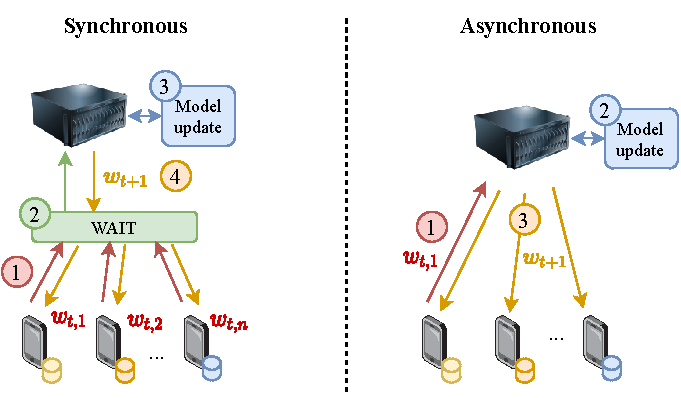
\includegraphics[width=.85\linewidth]{img/sync_vs_async_diagram.pdf}
	\caption{Synchronous vs asynchronous FL. Synchronous setting: (1) Local model update, (2) Wait, (3) Global model update, (4) Global model download. Asynchronous setting: (1) Local model update, (2) Global model update, (3) Global model download.}
	\label{fig:sync_vs_async_diagram}
\end{figure}

%As a result, BC may limit the performance of server-less FL applications, especially for a large number of participating clients. 
The introduction of BC to networking applications has, however, well-documented weaknesses~\cite{zheng2018blockchain}, including scalability, storage, and security aspects. To shed light on the feasibility of the BC-enabled FL approach, we provide an analytical model for characterizing the BC-enabled FL end-to-end latency. Based on this model, we provide an in-depth evaluation of the synchronous and the asynchronous BC-enabled server-less FL solutions and study the trade-off between the learning iteration time and the learning accuracy of each considered approach. While the synchronous solution grants high learning accuracy, the asynchronous one provides timely ML optimizations in large, heterogeneous deployments. In this regard, we also showcase the importance of the BC network capacity, which is essential for the proper execution of the consensus, on the FL end-to-end latency. The contributions of this paper are summarized as follows:
\begin{enumerate}
	\item We outline the use of BC to enable server-less FL applications (referred to as FLchain), which allows removing the need for a central server to orchestrate the learning operation in FL. Both synchronous (s-FLchain) and asynchronous (a-FLchain) training modes are explored.
	%
	\item We develop an analytical framework to derive the end-to-end latency associated with FLchain, which can be applied to both synchronous and asynchronous settings. A key aspect of the proposed framework is the batch-service queue model for measuring the queuing delay in a BC system, which is essential to capture asynchronous model update.
	%
	\item We study the effect that BC parameters have on the end-to-end training procedure in server-less FL.
	%
	\item We analyze the performance of s-FLchain and a-FLchain in terms of learning accuracy and completion time through simulations. For that, we use the well-known MNIST data set for hand-written characters recognition.
\end{enumerate}

%Our model is based on batch service queuing, so that batches of packets are served upon meeting certain conditions. This can be directly mapped to the BC operation, where blocks are filled with transactions before being mined. Based on the proposed model, we study the trade-off between the learning iteration time and the quality of an iteration in server-less FL. More specifically, we compare the synchronous and the asynchronous BC-enabled server-less FL solutions in terms of accuracy and learning completion latency. 

%In contrast, this might come at the cost of convergence guarantees. The fact is that asynchronous mechanisms are more challenging due to the high dynamics in them, which may potentially lead to a much higher number of iterations~\cite{dean2012large}. 

The rest of the paper is structured as follows: Section~\ref{section:related_work} overviews the related work on FLchain and queuing models for BC. Section~\ref{section:bc_fl} introduces aspects related to FL and BC technologies, as well as to their convergence to FLchain. Section~\ref{section:system_model} details the models used to characterize FLchain, for both synchronous and asynchronous training approaches. Section~\ref{section:delay_bc} provides the end-to-end latency framework for FLchain, including the batch service queue model for the BC queuing delay. In Section~\ref{section:results}, we evaluate the performance of s-FLchain and a-FLchain. Section~\ref{section:open} elaborates on the most promising open directions. Finally, Section~\ref{section:conclusions} concludes the paper.

%%%%%%%%%%%%%%%%%%%%%%%%%%%%
%% RELATED WORK
%%%%%%%%%%%%%%%%%%%%%%%%%%%%
\section{Related Work}
\label{section:related_work}

% FL ~\cite{li2021survey}
With the emergence of infrastructure-less network scenarios, the optimization carried out in FL is moving out of the central server to be handled in a decentralized manner~\cite{lalitha2018fully}. One of the first methods used to carry out server-less FL is based on the Gossip algorithm~\cite{blot2016gossip}, which has been applied for deep learning (DL) distributed training with remarkable success~\cite{hegedHus2021decentralized}. Other solutions such as the one presented in~\cite{chen2020wireless} advocate for hybrid settings, where clients can use device-to-device (D2D) links to aggregate information from nodes away from the base station (BS).

% FLChain
To enable server-less FL, BC technology has been introduced as an appealing solution, providing trust, transparency, and immutability~\cite{liu2020secure, al2021edge}. In this regard, the concept of \textit{FLchain} was firstly coined in~\cite{majeed2019flchain, bao2019flchain}, where BC was proposed to store model updates in blocks, therefore removing the figure of the central server. A systematic survey on FLchain can be found in~\cite{hou2021systematic}. FLchain has been embraced for 5G and beyond applications~\cite{lu2020blockchain2}, including use cases such as data sharing in industrial IoT~\cite{lu2019blockchain}, enabling data-driven cognitive computing in Industry 4.0~\cite{qu2020blockchained}, or enhancing trust in autonomous vehicles~\cite{pokhrel2020federated,qi2021privacy} (e.g., mobility verification, traffic prediction). A noteworthy implementation of an FLchain simulator has been provided in~\cite{qu2021chainfl} for edge computing environments. Additionally, an Ethereum-based implementation of FLchain was provided in~\cite{korkmaz2020chain}, which was evaluated through numerical results. As for the realization of FLchain, it has been envisioned to run over multiple architectural solutions, thus being empowered by paradigms like edge computing~\cite{majeed2019flchain}, fog computing~\cite{qu2020decentralized}, or peer-to-peer (P2P) communications~\cite{kim2019blockchained, ma2020federated}. 

%In healthcare, a blockchain-based FL application for COVID-19 detection has been proposed in~\cite{nguyen2021federated2}, thus embodying the privacy-preserving collaborative purpose of FLchain. 

% ASYNC FL
Regarding the training procedure in FLchain, most of the existing works consider synchronized approaches, which require gathering all the local model updates before generating a block. The FL iteration time is thus determined by the slowest user. Following the synchronous assumption, the FLchain performance may be deteriorated in heterogeneous networks, where devices have different communication and computation capabilities. Moreover, concerning the BC, generating large blocks (including information from a huge number of users) contributes to the instability of the BC, given that forks are more likely to occur as the block propagation time increases~\cite{wilhelmi2021performance}. As a result, including many synchronized local updates in a single block (as done in~\cite{kim2019blockchained,liu2021blockchain}) may lead to severe performance issues as the number of participating FL nodes increases.

When it comes to asynchronous training in FLchain, only a reduced number of contributions can be encountered in literature. In particular, the works in~\cite{lu2020blockchain, lu2020blockchain2} proposed a BC-enabled asynchronous FL solution for data sharing among vehicles. In this scenario, real-time communication becomes very challenging due to vehicles' unavailability and potential bandwidth constraints, so that asynchronous operation is a better fit, compared to synchronous solutions. On the topic of asynchronous learning in traditional FL settings, we refer the interested author to the survey in~\cite{xu2021asynchronous} and references therein.
%, it was firstly introduced in~\cite{keuper2015asynchronous}. Under this setting, each client computes and submits local updates at different rates, independently from the rest of the participants. To the best of our knowledge, little research has been conducted to explore asynchronous FL operation (see~\ref{xu2021asynchronous} and references therein). In particular, we find the works in~\cite{lu2020blockchain, lu2020blockchain2}, which proposed a BC-enabled asynchronous FL solution for data sharing among vehicles. In this scenario, real-time communication becomes very challenging due to vehicles' unavailability and potential bandwidth constraints, so the asynchronous operation fits better. %Moreover, the solution proposed in~\cite{lu2020blockchain, lu2020blockchain2} relies on the proper selection of the best nodes in terms of computational capacity and richest data partitions.

% Delay analysis
As for the performance evaluation of FLchain, several works can be found, which provide analytical and simulation results of the network overhead and training completion latency. In~\cite{kim2019blockchained}, an end-to-end latency model is provided by identifying the necessary steps both for FL (compute model updates, transmit updates, and model aggregation) and BC (mining, validation, and block propagation). Similarly, the work in~\cite{pokhrel2020federated} follows a step analysis to derive the delay incurred by the BC to FL training. Another relevant work is~\cite{feng2021blockchain}, which analyzes the transaction confirmation latency of an asynchronous BC-enabled FL application for IoT. Differently, the work in~\cite{lu2020low} analyzes the communication cost of FLchain and provides a deep reinforcement learning mechanism to improve a utility function that captures the trade-off between the learning time and the learning accuracy. Some of the abovementioned works rely on the synchronization of devices and miners in each FL step, including local and global model updates. Such a requirement leads to disregarding the queuing time associated with asynchronous training, which has a strong impact on the transaction confirmation time. To properly capture the impact of BC on FL, a deeper analysis of the FLchain end-to-end latency is required. 

Similarly to what we previously proposed in~\cite{wilhelmi2021discrete}, in this paper, we develop a novel batch-service queue model to characterize the latency of FLchain. Blockchain queue theory is an emerging field that has been recently introduced in~\cite{kawase2017transaction}, followed by the approaches in~\cite{kawase2018batch, li2018blockchain, geissler2019discrete}. The work in~\cite{kawase2017transaction} proposed a batch service queue model to understand the stochastic behavior of the transaction-confirmation process in Bitcoin. In a batch service queue, packets leave the queue in batches, rather than individually. This property is useful to capture the transactions life-cycle in a BC, which are gathered before being served (mined). The batch-service queue approach has been further extended and evaluated in~\cite{kawase2018batch, li2018blockchain}. Unlike the existing literature in batch-service queuing, our model characterizes timers and forks. While timers are employed to guarantee a maximum time between mined blocks, forks are a direct consequence of the consensus protocol used by miners. As a result, disregarding the effects of timers and forks may lead to poor accuracy when deriving the BC queue status (e.g., the number of transactions in it) and the expected delay.

%Furthermore, the authors provide a closed-form expression of the optimal block generation rate ($\lambda^*$) that minimizes the end-to-end latency, which depends on the clients' activity. Similarly, the work in~\cite{pokhrel2020federated} follows a stepped analysis to derive the delay incurred by the BC to the FL operation. Another relevant work is~\cite{feng2021blockchain}, which analyzes the transaction confirmation latency and derives $\lambda^*$ using a genetic algorithm. Alternatively,~\cite{lu2020low} analyzes the communication cost of FLchain and provides a deep reinforcement learning mechanism to improve the utility, which captures the trade-off between the learning time and the learning accuracy. 

%%%%%%%%%%%%%%%%%%%%%%%%%%%%
%% SOLUTION PROPOSAL
%%%%%%%%%%%%%%%%%%%%%%%%%%%%
\section{Enabling Secure, Decentralized Federated Learning through Blockchain}
\label{section:bc_fl}

%In this section, we first overview FL and BC technologies. Then, we present the FLchain setting as a compelling solution for server-less FL.

\subsection{Federated Learning}
\label{section:federated_learning}
%In FL, a typically large number of clients or learners (from tens to millions) collaborates, each one using unshared local data, to train a global shared model (e.g., a supervised learning task). This is done by allowing clients to exchange model parameters, which are iteratively updated until convergence, under the orchestration of a central server. 

In FL, a server interacts with clients, so that a global model is iteratively optimized, based on local updates. In an FL iteration, the server pushes a global model (e.g., parameters) to a set of clients, which perform on-device training (e.g., training a neural network for several epochs, based on different local data partitions) and upload their model updates. Once model updates are collected and aggregated by the server, a new global update is calculated. More iterations are run until convergence.

Formally, the goal of a FL algorithm is to solve a supervised learning optimization problem in a distributed (federated) manner. To that purpose, a set of $\mathcal{K}=\{1,2,...,K\}$ clients attempt to simultaneously optimize the global model parameters $w\in \mathbb{R}^d$ by using their local data $\{x_k,y_k\}$ with size $N_k$. More specifically, clients' local losses, given by $l_k(w,x_k,y_k)$, are combined to minimize a global finite-sum cost function $l(\cdot)$:
\begin{equation}
\min_{w\in \mathbb{R}^d} l(w) = \min_{w\in \mathbb{R}^d} \sum_{k=1}^{K} \frac{N_k}{N} l_k(w,x_k,y_k)
\label{eq:1}
\end{equation}

%Newton method: \cite{shamir2014communication}
Originally, the model parameters were optimized using the distributed approximate Newton method~\cite{konevcny2016federated}. But then the federated averaging (FedAvg) method~\cite{mcmahan2017communication} was widely adopted due to its effectiveness for non-convex problems and to its ability to reduce the communication overhead for synchronized stochastic gradient descent (SGD). In FedAvg, FL clients run multiple epochs of SGD before sending their locally computed gradients to the server, which updates the global model accordingly. Beyond FedAvg, other optimization mechanisms have been proposed to improve on convergence and efficiency aspects~\cite{reddi2020adaptive}.

% CONVERGENCE FL
Another important aspect of federated optimization lies in the communication with/among clients (either for client-server or decentralized D2D architectures), as convergence depends on the acceptance of a general model over a typically high number of different local distributions. For synchronized methods to achieve consensus, assumptions such as IIDness (statistical heterogeneity on clients' data) or strong convexity of the loss function (to be twice-continuously differentiable) are typically required~\cite{chen2020convergence,li2018federated,wang2019adaptive}. However, these properties may not hold in more challenging scenarios, where data sets are heterogeneous, clients' availability is highly variable, or updates are provided asynchronously~\cite{xie2019asynchronous,chen2020asynchronous}. Under these circumstances, it is challenging to provide convergence proofs, but several works advocate for speeding up performance through complementary tools like estimating the missing local updates through DL~\cite{chen2020convergence}. %In~\cite{chen2020convergence}, for instance, the authors provided a probabilistic model for reducing the training convergence time in a situation whereby not all the users can upload local updates concurrently, due to communication limitations. In particular, the lack of information at a given learning iteration is supplied by an artificial neural network (ANN) model that estimates the missing local updates. 

%%% BLOCKCHAIN
\subsection{Blockchain technology}
%BC, which was first introduced to empower decentralized transactions of cryptocurrencies~\cite{nakamoto2019bitcoin}, is a peer-to-peer technology for collaboratively sharing data in a secure, transparent, and traceable manner. More recently, with the irruption of smart contracts~\cite{szabo1994smart}, self-executable pieces of code that allow the automation of agreements among untrusted parties in a reliable manner, the application range of BC increased overwhelmingly, and reaching sectors like finance~\cite{guo2016blockchain}, healthcare~\cite{mettler2016blockchain}, governance~\cite{bohme2015bitcoin}, or telecommunications~\cite{nguyen2020blockchain}. The new paradigm of programmable trust impulsed by smart contracts allows reducing the operational costs caused by a traditional trust in third parties so that the different non-trusting parties can securely interact with each other. In telecommunications, BC has been identified as a powerful tool for efficient network operation and management, and as a potential enabler for trading resources as-a-service. Combined with artificial intelligence (AI), BC has become a striking enabler for network automation~\cite{liu2020blockchain, giupponi2021blockchain}.

Blockchain is a type of distributed ledger technology (DLT) that collects information in the form of transactions, which are gathered in blocks that are chained one after the other based on advanced cryptographic techniques. In essence, each block uses the hash value from the previous block to define its own structure (the first block is referred to as genesis block), thus leading to a tampered-proof sequence of information. To agree on the status of the chain (e.g., adding a new block), a set of participating nodes (typically referred to as miners) apply certain predefined consensus mechanisms (e.g., solving a mathematical puzzle), which is commonly referred to as mining. The implementation of consensus mechanisms ensures that any malicious change on data (e.g., for double-spending purposes) would not be accepted by the majority.

Fig.~\ref{fig:blockchain_summary} summarizes the steps carried out to add transactions to a BC. First (\textit{point 1}, in blue), users submit transactions to the miners' P2P network, which are responsible for verifying and propagating them to the rest of the miners (\textit{point 2}, in red). Once a new block is ready to be appended to the BC, miners run a given consensus algorithm for deciding the node responsible for updating the chain (\textit{point 3}, in green). Due to the distributed nature of the consensus algorithm, forks may occur if two or more miners come across the solution of a block at the same time, which leads to a conflict. When a fork occurs, the longest chain prevails and invalidates the transactions included in secondary chains.

\begin{figure}[ht!]
	\centering
	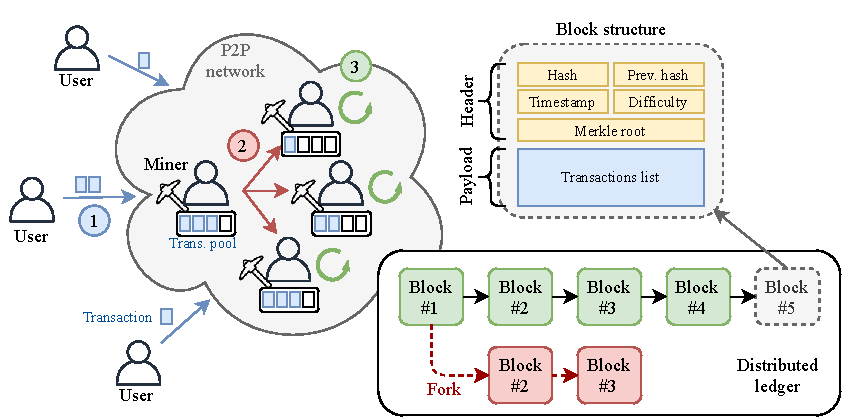
\includegraphics[width=\linewidth]{img/blockchain_summary.pdf}
	\caption{Overview of the procedure for mining transactions in a BC.}
	\label{fig:blockchain_summary}
\end{figure}

As noticed, the consensus is the core of BC technology, since it allows for securely and reliably exchanging data in a decentralized (and sometimes unreliable) network. Some of the most important consensus protocols are Proof-of-Work (PoW)~\cite{nakamoto2019bitcoin}, Proof-of-Stake (PoS)~\cite{saleh2021blockchain}, Practical Byzantine Fault Tolerance (PBFT)~\cite{castro1999practical}, or Ripple~\cite{schwartz2014ripple}. Throughout this work, we focus on PoW since it provides a high level of decentralization and raises interesting challenges in large-scale BC deployments.

\subsection{Blockchain for Federated Learning (FLchain)}
\label{section:flchain}

The realization of decentralized (server-less) FL through BC technology is often referred to as \textit{FLchain}~\cite{majeed2019flchain,nguyen2021federated}. In FLchain, FL devices exchange local information (e.g., gradients) through a BC, which keeps track of the individual model updates and allows performing model aggregation without using a central server (see Fig.~\ref{fig:blockchain_federated_learning}). Notice that the global model can be built either by the clients or by some intermediary nodes (e.g., edge servers acting as miners), which allows for a fully decentralized learning procedure. In~\cite{kim2019blockchained}, for instance, the local FL model updates are included in blocks, to be later aggregated by individual devices. In contrast, in~\cite{ma2020federated}, local updates are first spread and pre-processed by miners using Gossip, and then global updates are recorded in blocks. %The current literature on FLchain typically assumes that the data stored in the BC is perfectly shared among all the FL participants. However, as seen in~\cite{savazzi2020federated}, multiple synchronization problems may arise when exchanging model updates, thus requiring more sophisticated communication strategies (e.g., exchange local updates with a limited number of neighbor devices). 

\begin{figure}[ht!]
	\centering
	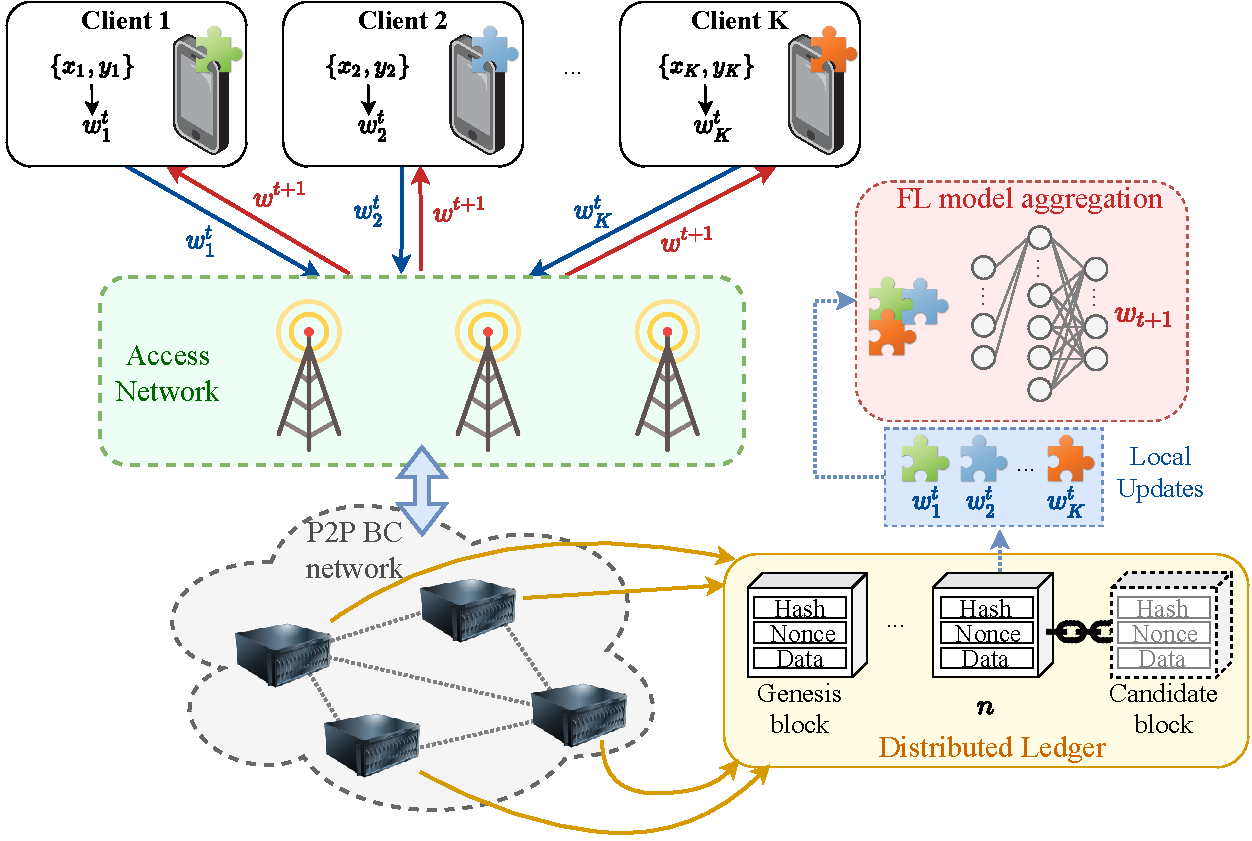
\includegraphics[width=\linewidth]{img/blockchain_federated_learning2.pdf}
	\caption{Decentralized FL enabled by BC technology.}
	\label{fig:blockchain_federated_learning}
\end{figure}

Taking into account the integration of BC into the FL operation, we identify the following iterative steps, which are executed either synchronously or asynchronously:
\begin{enumerate}
	\item \textbf{Local computation:} using local data, each client updates the model parameters by running a certain optimization mechanism (e.g., SGD).
	\item \textbf{Transactions gathering:} the local updates generated by clients are sent to miners and spread throughout the entire P2P network.
	\item \textbf{Block generation:} once enough valid transactions are collected (determined by the maximum block size), or if a maximum waiting time is exceeded, a candidate block is generated to be mined.
	\item \textbf{Block mining:} a consensus mechanism (e.g., solving a puzzle) is applied to decide the next block to be appended to the BC.
	\item \textbf{Block propagation:} after running a consensus mining algorithm, the mined block is propagated throughout the P2P network.
	\item \textbf{Global model aggregation:} using the information included in accepted blocks (i.e., local model updates), a global model update is derived. This step could be done locally or by devices with enough computational power (e.g., edge servers). In~\cite{kim2019blockchained,ma2020federated}, for instance, each client updates the global model by itself, unlike the case in Fig.~\ref{fig:blockchain_federated_learning}.
	\item \textbf{Block download:} clients download the latest block from the closest miner, which contain the global model update, $w^{t+1}$.
\end{enumerate}

In s-FLchain, the global model is initially downloaded by clients and then optimized in parallel, based on local data. Once all the local updates are uploaded to the BC network, a new block is generated and mined. The latest block contains all the local updates for updating the global model in a new iteration, so the block size ($S_\text{B}$) needs to be adapted to accommodate all of them. In a-FLchain, in contrast, clients perform local computation and submit local updates asynchronously. A new block is generated when the maximum block size ($S_\text{B}$) is reached, or when a predefined waiting timer ($\tau$) expires. %When receiving the updated global model, clients can decide whether to continue with the current local computation (with a previous version of the model) or to start a new one with the updated parameters. A staleness coefficient $\rho$ can be used for that purpose.

As noticed, the block size is an important parameter in FLchain. Setting it properly may have a high impact on the BC's throughput and, in consequence, on the FL completion time. In particular, the larger the block size, the higher the quality of the information provided in a single FL iteration, but the higher the fork probability and the transaction confirmation latency. Optimizing the optimal block size is a complex task that requires attention since it poses a trade-off between the block propagation delay and the fork probability. The optimization of the block size is out of the scope of this paper and is left as future work.

%%%%%%%%%%%%%%%%%%%%%%%%%%%%
%% SYSTEM MODEL
%%%%%%%%%%%%%%%%%%%%%%%%%%%%
\section{System Model}
\label{section:system_model}

%In this section, we present the learning, communication, and BC models used to characterize FLchain.

\subsection{Federated Learning Model}
\label{section:fl_model}

Let $\mathcal{K}$ (with size~$K=|\mathcal{K}|$) be a set of clients or learners attempting to optimize a global model $w \in \mathbb{R}^d$ by minimizing a loss function $l(w)$. Each client $k\in \mathcal{K}$ has a local data set $\{x_k,y_k\}$ with features and labels of size $N_k$, which is a subset of the entire data set (of size $N$) available across all the clients $\mathcal{X}\cup_{k=1}^K \{x_k,y_k\}$. During $t\in 1,2,...,T$ iterations, a subset of clients $\mathcal{K}_t \in \mathcal{K}$ with computational power $\xi_k^\text{FL}$ is sampled to compute local model updates $w_k^{t+1}, \forall k\in \mathcal{K}_t$, which are later aggregated to provide a global model update $w^{t+1}$. The FL operation stops after an arbitrary horizon or when $|l(w^t) - l(w^{t-1})| \leq \varepsilon$, being $\varepsilon \in \mathbb{R}$ a small error tolerance constant.

FedAvg with SGD is applied to compute the global model parameters. Under this setting, clients run $E$ epochs of SGD on their local data. In the traditional FL setting, local updates are sent to the server. In contrast, for FLchain, the updates are included in candidate blocks to be mined. For a single epoch, the local model parameters are updated by client $k$ as follows:
\begin{equation}
w_k^{t+1} = w^t - \eta_l \nabla l_{k}(w^t,x_k,y_k),
\label{eq:2}
\end{equation}

where $\eta_l$ is the learning rate for local updates (we use $\eta$ for global updates), and $\nabla l_{k}(w^t,x_k,y_k)$ is the average loss gradient of client $k$, based on the local data set $\{x_k,y_k\}$, with respect to the global model $w^t$. 

Upon receiving local updates, aggregation is done and the global model is updated by running a gradient-based global optimizer. More specifically, FedAvg updates the global model weights as follows:
\begin{equation}
w^{t+1} = \sum_{k\in \mathcal{K}_t} \frac{N_k}{N} w_{k}^{t+1}
\label{eq:3}
\end{equation}

The synchronous and the asynchronous versions of FLchain, s-FLchain and a-FLchain, are described in detail in Algorithm~\ref{alg:sflchain} and Algorithm~\ref{alg:aflchain}, respectively.

\begin{algorithm}[ht!]	
	\SetAlgoLined
	%	\KwIn{Error tolerance $\varepsilon$} 
	\textbf{Initialize:} $t=1$, $\eta_l$, $\eta$, $w^t = w^0$, $\varepsilon$\\
	\While{$|l(w^t) - l(w^{t-1})| > \varepsilon$}{
		$\mathcal{K}_t \sim \mathcal{U}(\mathcal{K})$ \Comment{sample random clients from $\mathcal{K}$} \\ 
		\For{$\forall k\in \mathcal{K}_t$ \text{(in parallel)}}{
			Download $w^t$\\
			$w^{t+1}_k \leftarrow$ LocalUpdate($w^t$, $\eta_l$, $x_k$, $y_k$)\\
			SubmitLocalUpdate($S_\text{tr}$, $C_k$)
		}
		%\eIf{\# received updates = $K$}
		%{
		MineBlock($\lambda$, $\xi^\text{M}$)\\
		PropagateBlock($S_\text{B}$, $C_\text{P2P}$)\\
		$w^{t+1}_k \leftarrow$ GlobalUpdate($w^t$, $w_k^{t+1}$, $\eta$)\\
		$ t \gets t + 1$
		%}{
		%    Wait()
		%}
	}
	\textbf{LocalUpdate}($w^t$, $E$, $\eta_l$, $x_k$, $y_k$): $E$ epochs of SGD are executed to optimize $l_k(\cdot)$\\
	\textbf{GlobalUpdate}($w^t$, $w_k^{t+1}$, $\eta$): the server aggregates the local updates $w_k^{t+1}$ to generate a global model $w^t$ \\
	\textbf{SubmitLocalUpdate}($S_\text{tr}$, $C^{}_k$): transactions with size $S_\text{tr}$ are sent through a link with capacity $C^{}_k$\\
	\textbf{MineBlock}($\lambda$, $\xi^\text{M}$): blocks are mined with block generation rate $\lambda$\\
	\textbf{PropagateBlock}($S_\text{B}$, $C_\text{P2P}$): blocks with size $S_\text{B}$ are sent through a link with capacity $C_\text{P2P}$\\
	\caption{Implementation of s-FLchain}
	\label{alg:sflchain}			
\end{algorithm}

\begin{algorithm}[ht!]	
	\SetAlgoLined
	\textbf{Initialize:} $t=1$, $\eta_l$, $\eta$, $w^t = w^0$, $\varepsilon$\\
	\While{$|l(w^t) - l(w^{t-1})| > \varepsilon$}{
		\textbf{Clients (asynchronously):}\\
		Download $w^t$\\
		$w^{t+1}_k \leftarrow$ LocalUpdate($w^t$, $\eta_l$, $x_k$, $y_k$)\\
		$u^t_k \leftarrow$ SubmitLocalUpdate($S_\text{tr}$, $C_k$)\\
		\textbf{Blockchain (in parallel):}\\
		\eIf{$|u^t| \geq S_\text{B}$ or $\tau$ has expired}
		{
			MineBlock($\lambda$, $\xi^\text{M}$)\\
			PropagateBlock($\min(|u_t|,S_\text{B}$), $C_\text{P2P}$)\\
			$w^{t+1}_k \leftarrow$ GlobalUpdate($w^t$, $w_k^{t+1}$, $\eta$)\\
			$ t \gets t + 1$\\
			Restart $\tau$
		}{
			Wait
		}
	}
	\textbf{LocalUpdate}($w^t$, $E$, $\eta_l$, $x_k$, $y_k$): $E$ epochs of SGD are executed to optimize $l_k(\cdot)$\\
	\textbf{GlobalUpdate}($w^t$, $w_k^{t+1}$, $\eta$): the server aggregates the local updates $w_k^{t+1}$ to generate a global model $w^t$ \\
	\textbf{SubmitLocalUpdate}($S_\text{tr}$, $C^{}_k$): transactions with size $S_\text{tr}$ are sent through a link with capacity $C^{}_k$\\
	\textbf{MineBlock}($\lambda$, $\xi^\text{M}$): blocks are mined with block generation rate $\lambda$\\
	\textbf{PropagateBlock}($S_\text{B}$, $C_\text{P2P}$): blocks with size $S_\text{B}$ are sent through a link with capacity $C_\text{P2P}$\\  
	\caption{Implementation of a-FLchain}
	\label{alg:aflchain}			
\end{algorithm}

\subsection{Communication Model}
\label{section:comm_model}
We consider $P$ orthogonal wireless channels under frequency division multiple access (FDMA) for supporting the communication among clients and peer nodes. For a given transmitter-receiver pair $\{i,j\}$, the data rate of the link $R_{i,j}$, depends on the bandwidth $b_{i}$ allocated to the transmitter and the signal-to-interference-plus-noise ratio (SINR), $\gamma_{j}$, at the receiver:   
\begin{equation}
R_{i,j} = b_i \log_2(1 + \gamma_j)
\end{equation}

The SINR at node $j$ can be expressed as follows:
\begin{equation}
\gamma_j = \frac{P_{i}G_{i,j}}{\sum_{\forall l \neq i,j}P_l G_{l,j} +\sigma_0},
\end{equation}

where $P_{i}$ is the power used by transmitter $i$, $G_{i,j}$ is the channel gain, and $\sigma_0$ is the noise power. Regarding the path-loss model, the loss at distance $d$ is given by:%~\cite{feng2006path,fryziel2002path}:
\begin{equation}
PL(d) = P_t-PL_0+10 \alpha \log_{10}(d) + \frac{\sigma}{2} + \frac{d}{10} \frac{\zeta}{2},
\end{equation}

where $P_t$ is the power at the output of the transmitter's antenna, $PL_0$ is the loss at the reference distance, $\alpha$ is the path-loss exponent, $\sigma$ is the shadowing factor, and $\zeta$ is the obstacles factor. %As for the links between miners in the P2P network, we consider wired X2/Xn interfaces with fixed latency (e.g., 10~ms).

\subsection{Blockchain Model}
\label{section:bc_model}

We consider a public BC for publishing the FL local parameters in the form of transactions, each of size $S_\text{tr}$, to be aggregated in blocks of size $S_\text{B}$ (including headers). The P2P network maintaining the BC is formed by $M$ miners, each one running PoW in parallel. In PoW, the first miner to correctly solve and propagate the answer of a puzzle is allowed to append a block to the BC. Other consensus mechanisms in the literature~\cite{nguyen2018survey} suit a wide range of applications (e.g., public/private governance, small/big P2P networks, high/low transparency, etc.), but PoW grants a high degree of decentralization and offers robustness in massively operated BCs. For further discussion on different consensus mechanisms refer to Section~\ref{section:consensus}.%Nevertheless, we stick to PoW for the performance evaluation of this work and leave the analysis for the rest of the methods as future work. A more in-depth discussion on different consensus mechanisms is provided in Section~\ref{section:consensus}.

As a result of the PoW operation, the performance of the BC can be hindered by forks. A fork is a split of the BC into different states, and can potentially compromise the overall agreement among participants, and thus threaten stability. Forks typically occur when two or more miners solve the nonce of a candidate block almost simultaneously, i.e., before the block has been propagated by a single miner. For a fixed mining difficulty ($D$) and miners' computational power ($\xi_m^\text{M}$), assuming the synchronous operation of $M$ miners and given the block propagation delay $\delta_\text{bp}$ (see the following sections for more details), we define the fork probability as:
\begin{equation}
\begin{split}
p_\text{fork} = 1 - e^{-\lambda(M-1)\delta_\text{bp}}
%&= 1 - \prod_{\forall i \neq w} \Pr(T_\text{bg}(i) - T_\text{bg}(w) > T_\text{bp}) \\&= 1 - e^{-\mu (M-1)T_\text{bp}},
%\nonumber
\end{split}
\label{eq:fork_probability}
\end{equation}

Note that the mining procedure, as widely adopted in the literature~\cite{decker2013information}, follows an exponential distribution with parameter $\lambda$ (the expected block generation time is $1/\lambda$), so the time between mined blocks can be represented by a Poisson inter-arrival process. %The block generation rate depends on the mining difficulty ($D$) and the miners' computational power ($\xi_m^\text{M}$). Based on this last parameter, Bitcoin's BC adapts the PoW difficulty to maintain an average mining time of ten minutes. 

In s-FLchain, miners must wait for all the local updates before building a block. As for a-FLchain, the waiting time is affected by the transaction arrivals and the maximum waiting time $\tau$, among other parameters. In particular, we model the arrivals process through a Poisson distribution with parameter $\nu$, which is a function of the clients' activity (it depends on the size of their local data sets and their computation and communication capabilities). We define $\nu$ as follows:%\textcolor{red}{[this function needs to be defined]}:
\begin{equation}
% \sum_{k=1}^{K} f(x_k, \xi^\text{FL}_k, R_{i,j}) =
\nu = \sqrt{K \Bigg( \min_{m\in \mathcal{M}} \frac{1}{K} \sum_{k=1}^{K} \Big( \frac{S_\text{B}}{R_{m,k}} + |x_k|\xi^\text{FL} + \frac{S_\text{tr}}{R_{k,m}} \Big) \Bigg)^{-1}},
\end{equation}

where $\xi^\text{FL}$ is the required amount of CPU cycles to process a single FL training data point and $S_\text{tr}$ is the size of a transaction including a client's local update. We would like to remark that the parameter $\nu$ is hard to estimate because it depends on the transaction confirmation latency, which also depends on $\nu$. Notice that submitting a transaction (a model update) to the BC is a blocking process from the point of view of a single node: once a transaction is submitted, it needs to wait until the next mined block before generating a new local update (a global model update is required before computing and submitting the next local update). %This includes queue time, block generation, block propagation, and model aggregation. Therefore, the higher the initial $\nu$, the higher the time between blocks.

%%%%%%%%%%%%%%%%%%%%%%%%%%%%
%% ANALYSIS
%%%%%%%%%%%%%%%%%%%%%%%%%%%%
\section{Delay Analysis of Blockchain-enabled Federated Learning}
\label{section:delay_bc}

%In this section, we analytically derive the latency incurred by the proposed FLchain mechanisms. A novel batch-service queue model is provided for the characterization of the latency.

\subsection{FLchain iteration latency}

To measure the necessary time to perform the s-FLchain and a-FLchain procedures defined in Section~\ref{section:flchain}, we identify the following delays:
\begin{enumerate}
	\item \textbf{Block filling delay ($\delta_\text{bf}$)}: a block is filled with transactions (i.e., local updates) from clients. This includes local model computation (clients run gradient descent on their own data set to update the local model) and local model upload (clients submit their local updates to the closest miner).
	%
	\item \textbf{Block generation delay ($\delta_\text{bg}$):} miners run PoW to find the block's nonce, or until receiving a new valid mined block.
	%
	\item \textbf{Block propagation delay ($\delta_\text{bp}$):} mined blocks are propagated throughout the entire P2P network. We assume that all the miners receive the propagated blocks simultaneously.
	%
	\item \textbf{Global model aggregation delay ($\delta_\text{agg}$):} a global model update is generated by aggregating the local updates from the latest mined block. The aggregation procedure can either be done by clients (fully decentralized) or by miners (edge computing-based). In case aggregation is performed by clients, the block download procedure is done first.
	%
	\item \textbf{Block download delay ($\delta_\text{bd}$):} clients download the latest propagated block from miners, containing either the local updates from the previous iteration or the updated global model, depending on the model aggregation approach.
\end{enumerate}

Gathering all the delays in FLchain, and by taking into account the negative implications of forks, we define the expected iteration time ($\text{T}_\text{iter}$) as:
\begin{equation}
\text{T}_\text{iter} =  \frac{(\delta_\text{bf} + \delta_\text{bg} + \delta_\text{bp})}{1-p_\text{fork}} + \delta_\text{agg} + \delta_\text{bd},
\label{eq:delay}
\end{equation}

Notice that the block filling, the block generation, and the block propagation operations are affected by forks. Therefore, these steps may potentially be repeated in case conflicts arise.

\subsection{Batch-service queue model for a-FLchain}

In s-FLchain, all the devices are assumed to be synchronized, so the time for gathering transactions in a block is deterministic and depends on the slowest node:
\begin{equation}
\delta_\text{bf}^\text{sync} = \max_{k\in \mathcal{K}} (\delta_\text{c}^k + \delta_\text{ul}^k),
\end{equation}
where $\delta_\text{c}^k$ and $\delta_\text{ul}^k$ are the local computation and local model upload delays, respectively, at the $k$-th client. These delays depend on each device's computation and communication capabilities. 

In contrast, in a-FLchain, transactions are collected asynchronously, following a random distribution that depends on the clients' activity. In particular, a block is generated when enough transactions have been collected by miners (which depends on the block size $S_\text{B}$), or when a maximum waiting time $\tau$ is exceeded. To capture the block filling latency in the asynchronous case, we focus on queue theory and derive the batch-service queue model illustrated in Fig.~\ref{fig:batch_service_queue}. As shown in the figure, the block filling procedure is determined by the block size $S_\text{B}$, the arrivals rate $\nu$, and by the maximum waiting time $\tau$. If the number of arrivals is enough for filling a block before $\tau$ expires, then a block with size $S_\text{B}$ is generated following PoW. Otherwise (the timer expires), a lower number of transactions than $S_\text{B}$ is included to the candidate block. 

\begin{figure}[ht!]
	\centering
	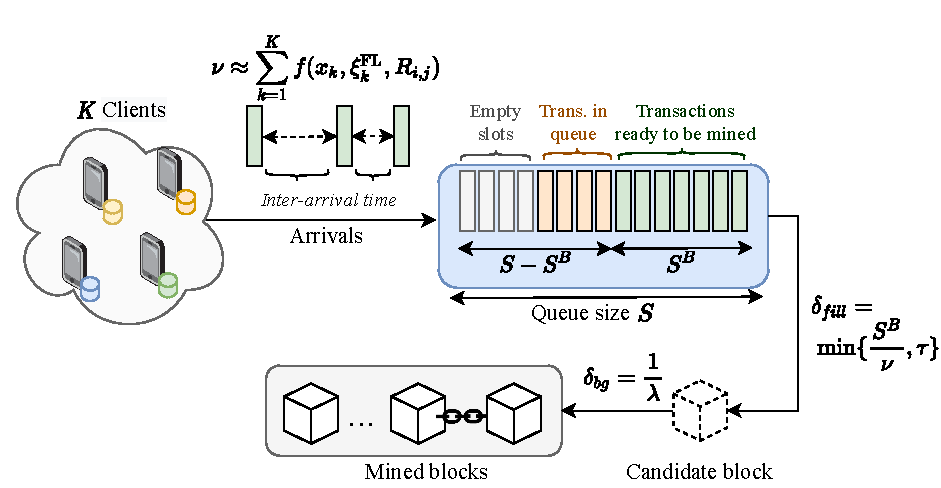
\includegraphics[width=\linewidth]{img/batch_service_queue2.pdf}
	\caption{Batch-service queue model for a-FLchain.}
	\label{fig:batch_service_queue}
\end{figure}

We model the states of a finite queue (with size $S$) at the departure states through a Markov chain, with states indicating the queue occupancy (number of transactions) just before a departure. In particular, the state of the batch service queue at the $n$-th departure instant is given by:
\begin{equation}
q_n = 
\min \Big\{ q_{n-1} + a(q_{n-1}) - d(q_{n-1}), S - d(q_{n-1}) \Big\},
\end{equation}
where $q_{n-1}$ is the state of the queue before the previous departure, $a(q_{n-1})$ is the number of new arrivals during the last inter-departure epoch, and $d(q_{n-1})$ is the number of packets delivered in a batch. The queue state after departures is illustrated in Fig.~\ref{fig:queue_arrivals_example}, which considers a simple example of a queue with $S_\text{B}=2$. 

\begin{figure}[ht!]
	\centering
	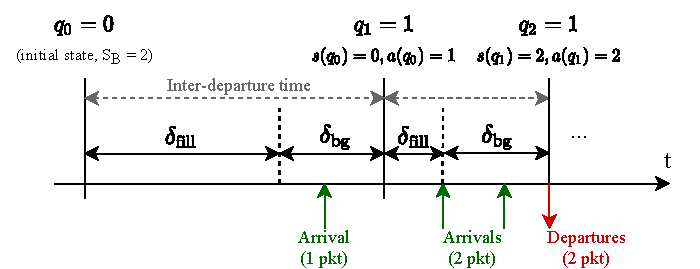
\includegraphics[width=\columnwidth]{img/queue_arrivals_example.pdf}
	\caption{Inter-departure states in a batch-service queue with $S_\text{B}=2$.}
	\label{fig:queue_arrivals_example}
\end{figure}

As shown int the figure, the queue status at the beginning is $q_0 = 0$ (the queue is empty). During the inter-departure time, we observe an arrival, which occurred during the block generation period. In this case, $\tau$ expired before noticing any arrival during the block filling time, thus no packets are included in the mined block. During the next inter-departure period (starting from $q_1 = 1$) we find one more arrival that completes the block, so block generation is performed before the timer expires. Finally, a new arrival is noticed during the mining time, so the queue ends up in $q_2 = 1$.

The departure probability distribution $\boldsymbol{\pi}^d$ is obtained by solving $\boldsymbol{\pi}^d = \boldsymbol{\pi}^d \boldsymbol{\text{P}}$ (with normalization condition $\boldsymbol{\pi}^d \boldsymbol{1}^T = 1$), where $\text{P}$ is the transition-probability matrix for departure states. Assuming that arrivals and departures follow independent Poisson and exponential distributions, respectively, the transition probabilities in $\text{P}$, for any pair of states $(i,j)$, are obtained as follows:
\begin{equation}
\resizebox{\linewidth}{!}{%
	$p_{i,j} = \begin{cases}
	\frac{\lambda}{\lambda + \nu} \Big(\frac{\nu}{\lambda + \nu}\Big)^{j-(i-d(i))}, & [i - d(i)]^+ \leq j < S - d(i)
	\\
	\\
	1-\sum^{S-d(i)-1}_{l=0} p_{i,l}, & j = S - d(i)
	\\
	\\
	0, & \text{otherwise}
	\end{cases}$
}
\end{equation}

Next, using the Poisson arrivals see time averages (PASTA) property, we obtain the steady-state queue distribution $\boldsymbol{\pi}^s$, which will later allow us to derive the expected queuing delay based on Little's law~\cite{shortle2018fundamentals}. From $\boldsymbol{\pi}^d$, we compute $\boldsymbol{\pi}^s$ for states $s < S$:
\begin{equation}
\begin{split}
\pi^s &= \frac{1}{\nu \text{E}[T]} \sum_{i=0}^s \pi_i^d \bigg( \overline{\varsigma_{\tau,i}} \Big( \sum_{j=s-d(i)+1}^{S-d(i)} p_{i,j} \Big) \\
&+ \varsigma_{\tau,i} \Big( \sum_{j=i}^{S_\text{B}-1} \text{P}(n=j-i|\tau) \big(\sum_{l=s-d(j-i)+1}^{S-d(j-i)} p_{j,l}\big) \Big) \bigg),
\end{split}
\end{equation}
where $\varsigma^{\tau}_i$ is the timer expiration probability from departure state $i$, which is non-zero for $i<S_\text{B}$. The steady-state probability of finding the queue full is given by $\pi^S = 1-\sum^{S-1}_{s=0} \pi^{s}$. Finally, the expected queue delay is computed as:
\begin{equation}
\delta_\text{bf}^\text{async} = \frac{\sum_{s=0}^S s \pi^s}{\nu(1-\pi^S)}
\end{equation}

Notice, as well, that all the transactions included in the block(s) involved in forks are added twice to the BC. This is a worst-case scenario that has implications in the queue occupancy, thus contributing to increasing the queuing delay. Nevertheless, the consistency among the set of transactions proposed by each miner relies on the underlying communication capabilities (i.e., how transactions are propagated throughout the P2P network), on the behavior of miners (e.g., malicious miners may temporarily hold transactions to mine the next block with higher probability), and on the incentives offered by each user willing to submit a transaction (e.g., paying a fee for including a transaction in the next block). Some future directions are provided in Section~\ref{section:consensus} in relation to this.

%\begin{equation} 
%    p_{\tau,i} = \sum_{j=i}^{S_\text{B}-1}  e^{-\nu \tau} \frac{(\nu \tau)^j}{j!}
%\end{equation}
%\begin{figure*}[!t]
%\begin{equation} \label{eq:pi_s}
%\pi_k^s = \begin{cases}
%    \frac{1}{\nu \text{E}[T]} \sum_{i=0}^k \pi_i^d \bigg( \overline{\varsigma}_{\tau,i} \Big( \sum_{j=k-d(i)+1}^{S-d(i)} p_{i,j} \Big) + \varsigma_{\tau,i} \Big( \sum_{j=i}^{S_\text{B}-1} \text{P}(n=j-i|\tau) \big(\sum_{l=k-d(j-i)+1}^{S-d(j-i)} p_{j,l}\big) \Big) \bigg), & k < S
%    \\
%    \\
%    1-\sum^{S-1}_{s=0} \pi_{i}^s, & s = S
%    \end{cases}
%\end{equation}
%\hrulefill
%\end{figure*}

%%%%%%%%%%%%%%%%%%%%%%%%%%%%
%% RESULTS
%%%%%%%%%%%%%%%%%%%%%%%%%%%%
\section{Performance Evaluation}
\label{section:results}

In this section, we evaluate the performance of FLchain and provide insights on its suitability.\footnote{All the source code used in this project is open-access and can be accessed at \url{www.github.com/fwilhelmi/blockchain_enabled_federated_learning}, commit: 648ead5. Accessed: November 30, 2021.} First, we analyze aspects of the BC and assess the sensitivity of this technology on various important parameters, such as the arrivals rate ($\nu$), the block size ($S_\text{B}$), or the block generation rate ($\lambda$). Then, we evaluate both s-FLchain and a-FLchain solutions. The simulation parameters are collected in Table~\ref{tab:sim_parameters}.

\begin{table}[ht!]
	\centering
	\caption{Simulation parameters.}
	\label{tab:sim_parameters}
	\resizebox{\columnwidth}{!}{\begin{tabular}{|c|c|l|c|}
			\hline
			\multicolumn{1}{|l|}{} & \textbf{Parameter} & \multicolumn{1}{c|}{\textbf{Description}} & \multicolumn{1}{c|}{\textbf{Value}} \\ \hline
			\multirow{5}{*}{\rotatebox{90}{\textbf{Blockchain}}} & $S_\text{tr}$ & Transaction size & 5 Kbits \\ \cline{2-4} 
			& $S_{h}$ & Block header size & 200 Kbits \\ \cline{2-4} 
			& $M$ & Number of miners & 10 \\ \cline{2-4} 
			& $\tau$ & Max. waiting time & 1,000 s \\ \cline{2-4} 
			& $S$ & Queue length & 1,000 \\ \hline
			% & $\xi^{M}$ & Mining computational power &
			\multirow{10}{*}{\rotatebox{90}{\textbf{Communication}}} & $d_{\min}/d_{\max}$ & Min/max distance client-BS & 0 / 4.15 m \\ \cline{2-4} 
			& $b$ & Bandwidth & 180 kHz \\ \cline{2-4} 
			& $F_c$ & Carrier frequency & 2 GHz \\ \cline{2-4} 
			& $G$ & Antenna gain & 0 dBi \\ \cline{2-4} 
			& $P_t$ & Transmit power & 20 dBm \\ \cline{2-4} 
			& $PL_0$ & Loss at the reference dist. & 5 dB \\ \cline{2-4} 
			& $\alpha$ & Path-loss exponent & 4.4 \\ \cline{2-4} 
			& $\sigma$ & Shadowing factor & 9.5 \\ \cline{2-4} 
			& $\zeta$ & Obstacles factor & 30 \\ \cline{2-4}
			& $\sigma_0$ & Ground noise & -95 dBm \\ \cline{2-4}
			& $C_\text{P2P}$ & Capacity P2P links & 5 Mbps \\ \hline
			\multirow{10}{*}{\rotatebox{90}{\textbf{Fed. Learning}}} & $\mathcal{A}$ & Learning algorithm & Neural Network \\ \cline{2-4} 
			& $h_l$ & Number of hidden layers & 2 \\ \cline{2-4} 
			& $a$ & Activation function & ReLU \\ \cline{2-4} & $o$ & Optimizer & SGD \\ \cline{2-4}
			& $l$ & Loss function & Cat. Cross-Entropy \\ \cline{2-4}
			& $\eta_l$/$\eta$ & Learning rate (local/global) & 0.01/1 \\ \cline{2-4}
			& $E$ & Epochs number & 5 \\ \cline{2-4}
			& $B$ & Batch size & 20 \\ \cline{2-4}
			& $\xi^\text{FL}$ & CPU cycles to process a data point & $10^{-5}$ \\ \cline{2-4}
			& $\xi^\text{FL}_k$ & Clients' clock speed & 1~GHz \\ \hline
		\end{tabular}
	}
\end{table}

%Time to process a single data point:  $\xi^\text{FL}/\xi^\text{FL}_i = 0.1$ ms

\subsection{Blockchain queue delay}

Fig.~\ref{fig:bc_delay_mu} shows the average queue performance, including the expected delay, average occupancy, and fork probability, for different block generation rates, block sizes, and user arrival rates. As expected, the queue occupancy decreases as $\lambda$ increases, which allows processing transactions faster. However, the fork probability also increases with $\lambda$, which may compromise the performance of the BC. %Some of these parameters depend on the FL problem (network size, updates per second, etc.), while some others are specific to the BC implementation. %For the sake of analyzing the effects that the studied parameters have on the BC performance, we have set $\tau$ to an arbitrary large value (i.e., 1,000 seconds).

\begin{figure}[ht!]
	\centering
	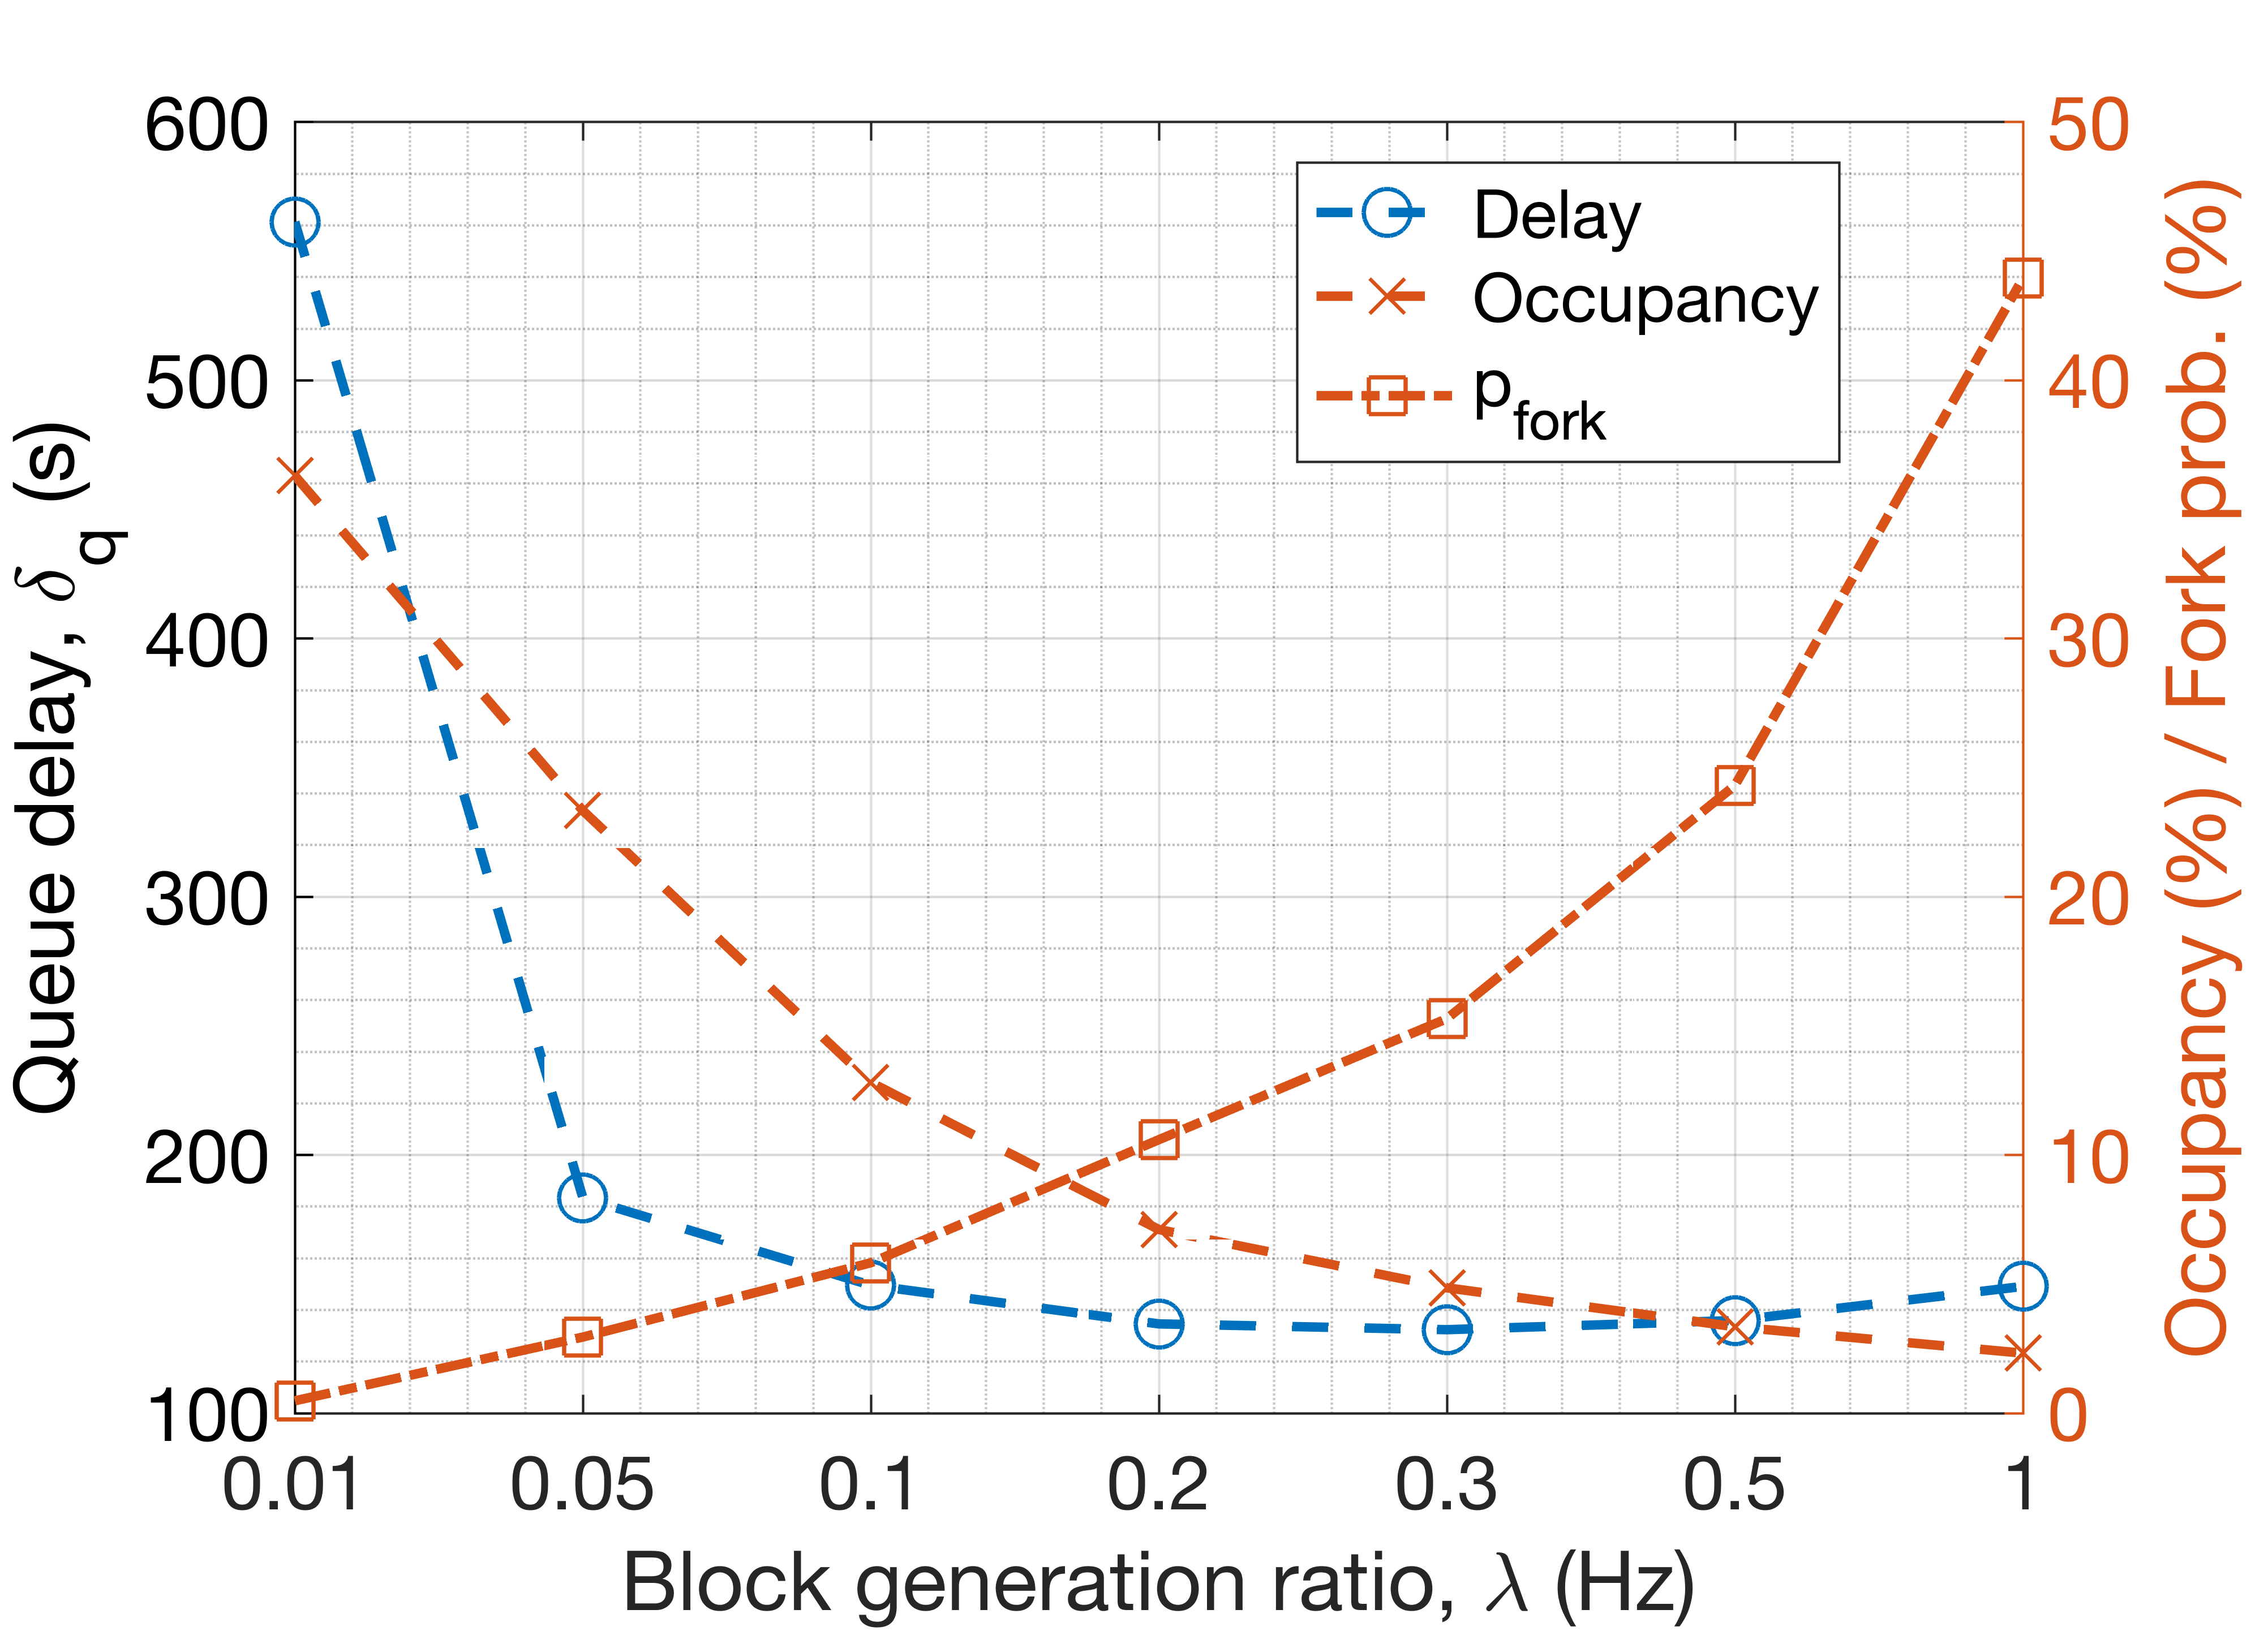
\includegraphics[width=.75\linewidth]{img/1_mean_occupancy_delay_2.png}
	\caption{Mean BC queuing delay as a function of $\lambda$. The queue occupancy and the fork probability ($p_\text{fork}$) are also plotted. Different user arrival rates $\nu$ and block sizes $S_\text{B}$ are considered and averaged in each data point.}
	\label{fig:bc_delay_mu}
\end{figure}

Alternatively, Fig.~\ref{fig:2_block_size_lambda02} analyzes the impact of the block size on the queuing delay, for representative $\nu$ (low and high traffic, respectively) and $\lambda$ values ($\{0.05, 0.2, 1\}$ Hz). As shown in the figure, the behavior of the queue delay differs for different $\nu$ values. On the one hand, for a high arrivals rate (e.g., $\nu = 20$), the queue delay is very high for short block sizes, as the queue is filled with transactions that cannot be delivered in time. The effect is the opposite for a few arrivals ($\nu = 0.02$), where the queue delay increases with the block size because the queued transactions need to wait until a block is filled.

\begin{figure}[ht!]
	\centering
	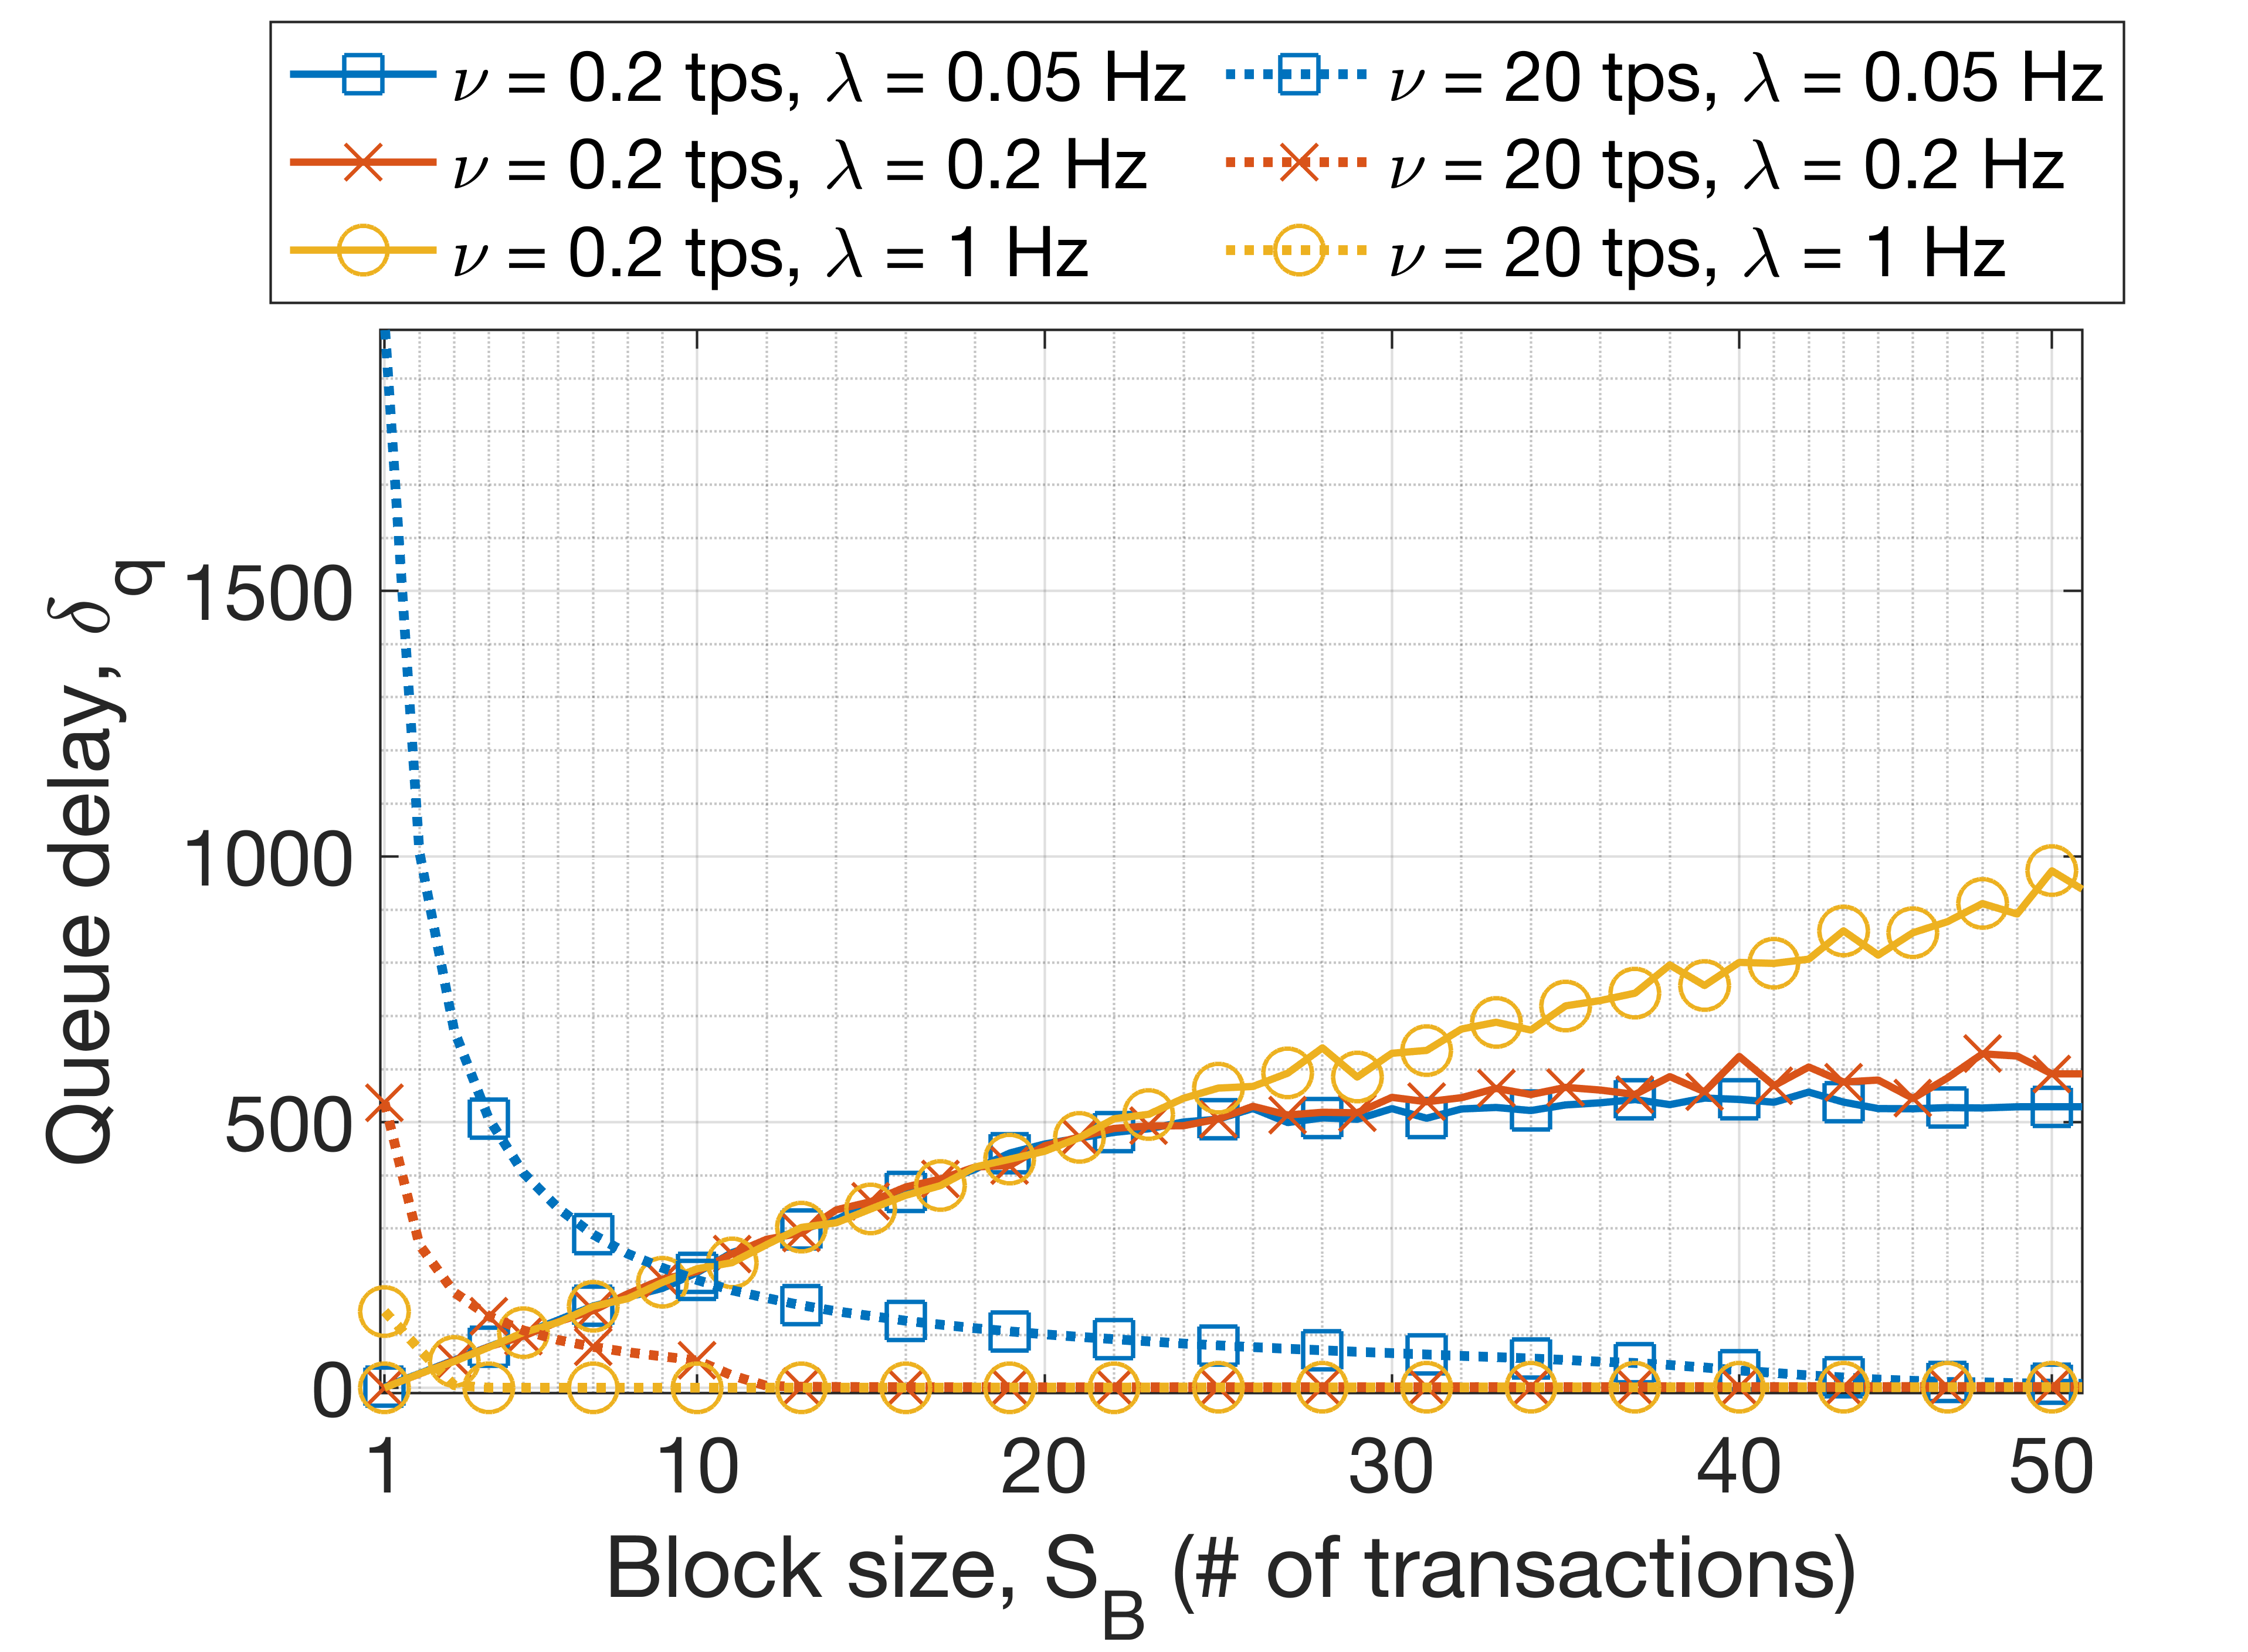
\includegraphics[width=.75\linewidth]{img/0_block_size_delay.png}
	\caption{BC queue delay as a function of the block size ($S_\text{B}$). Different $\nu$ (in transactions per second) and $\lambda$ values are considered.}
	\label{fig:2_block_size_lambda02}
\end{figure}

\subsection{Blockchain transaction confirmation latency}

We focus on the transaction confirmation latency, which includes transmission times (transaction and block propagation) and the re-transmissions caused by forks, as captured in \eqref{eq:delay}. Fig.~\ref{fig:4_transaction_confirmation_delay} illustrates the BC's average transaction confirmation latency ($\text{T}_\text{BC}$), together with the fork probability, for different block generation rates. In addition, different BC P2P network capacities have been displayed, including capacities of $C_\text{P2P}=\{5, 20, 50\}$~Mbps.

\begin{figure}[ht!]
	\centering
	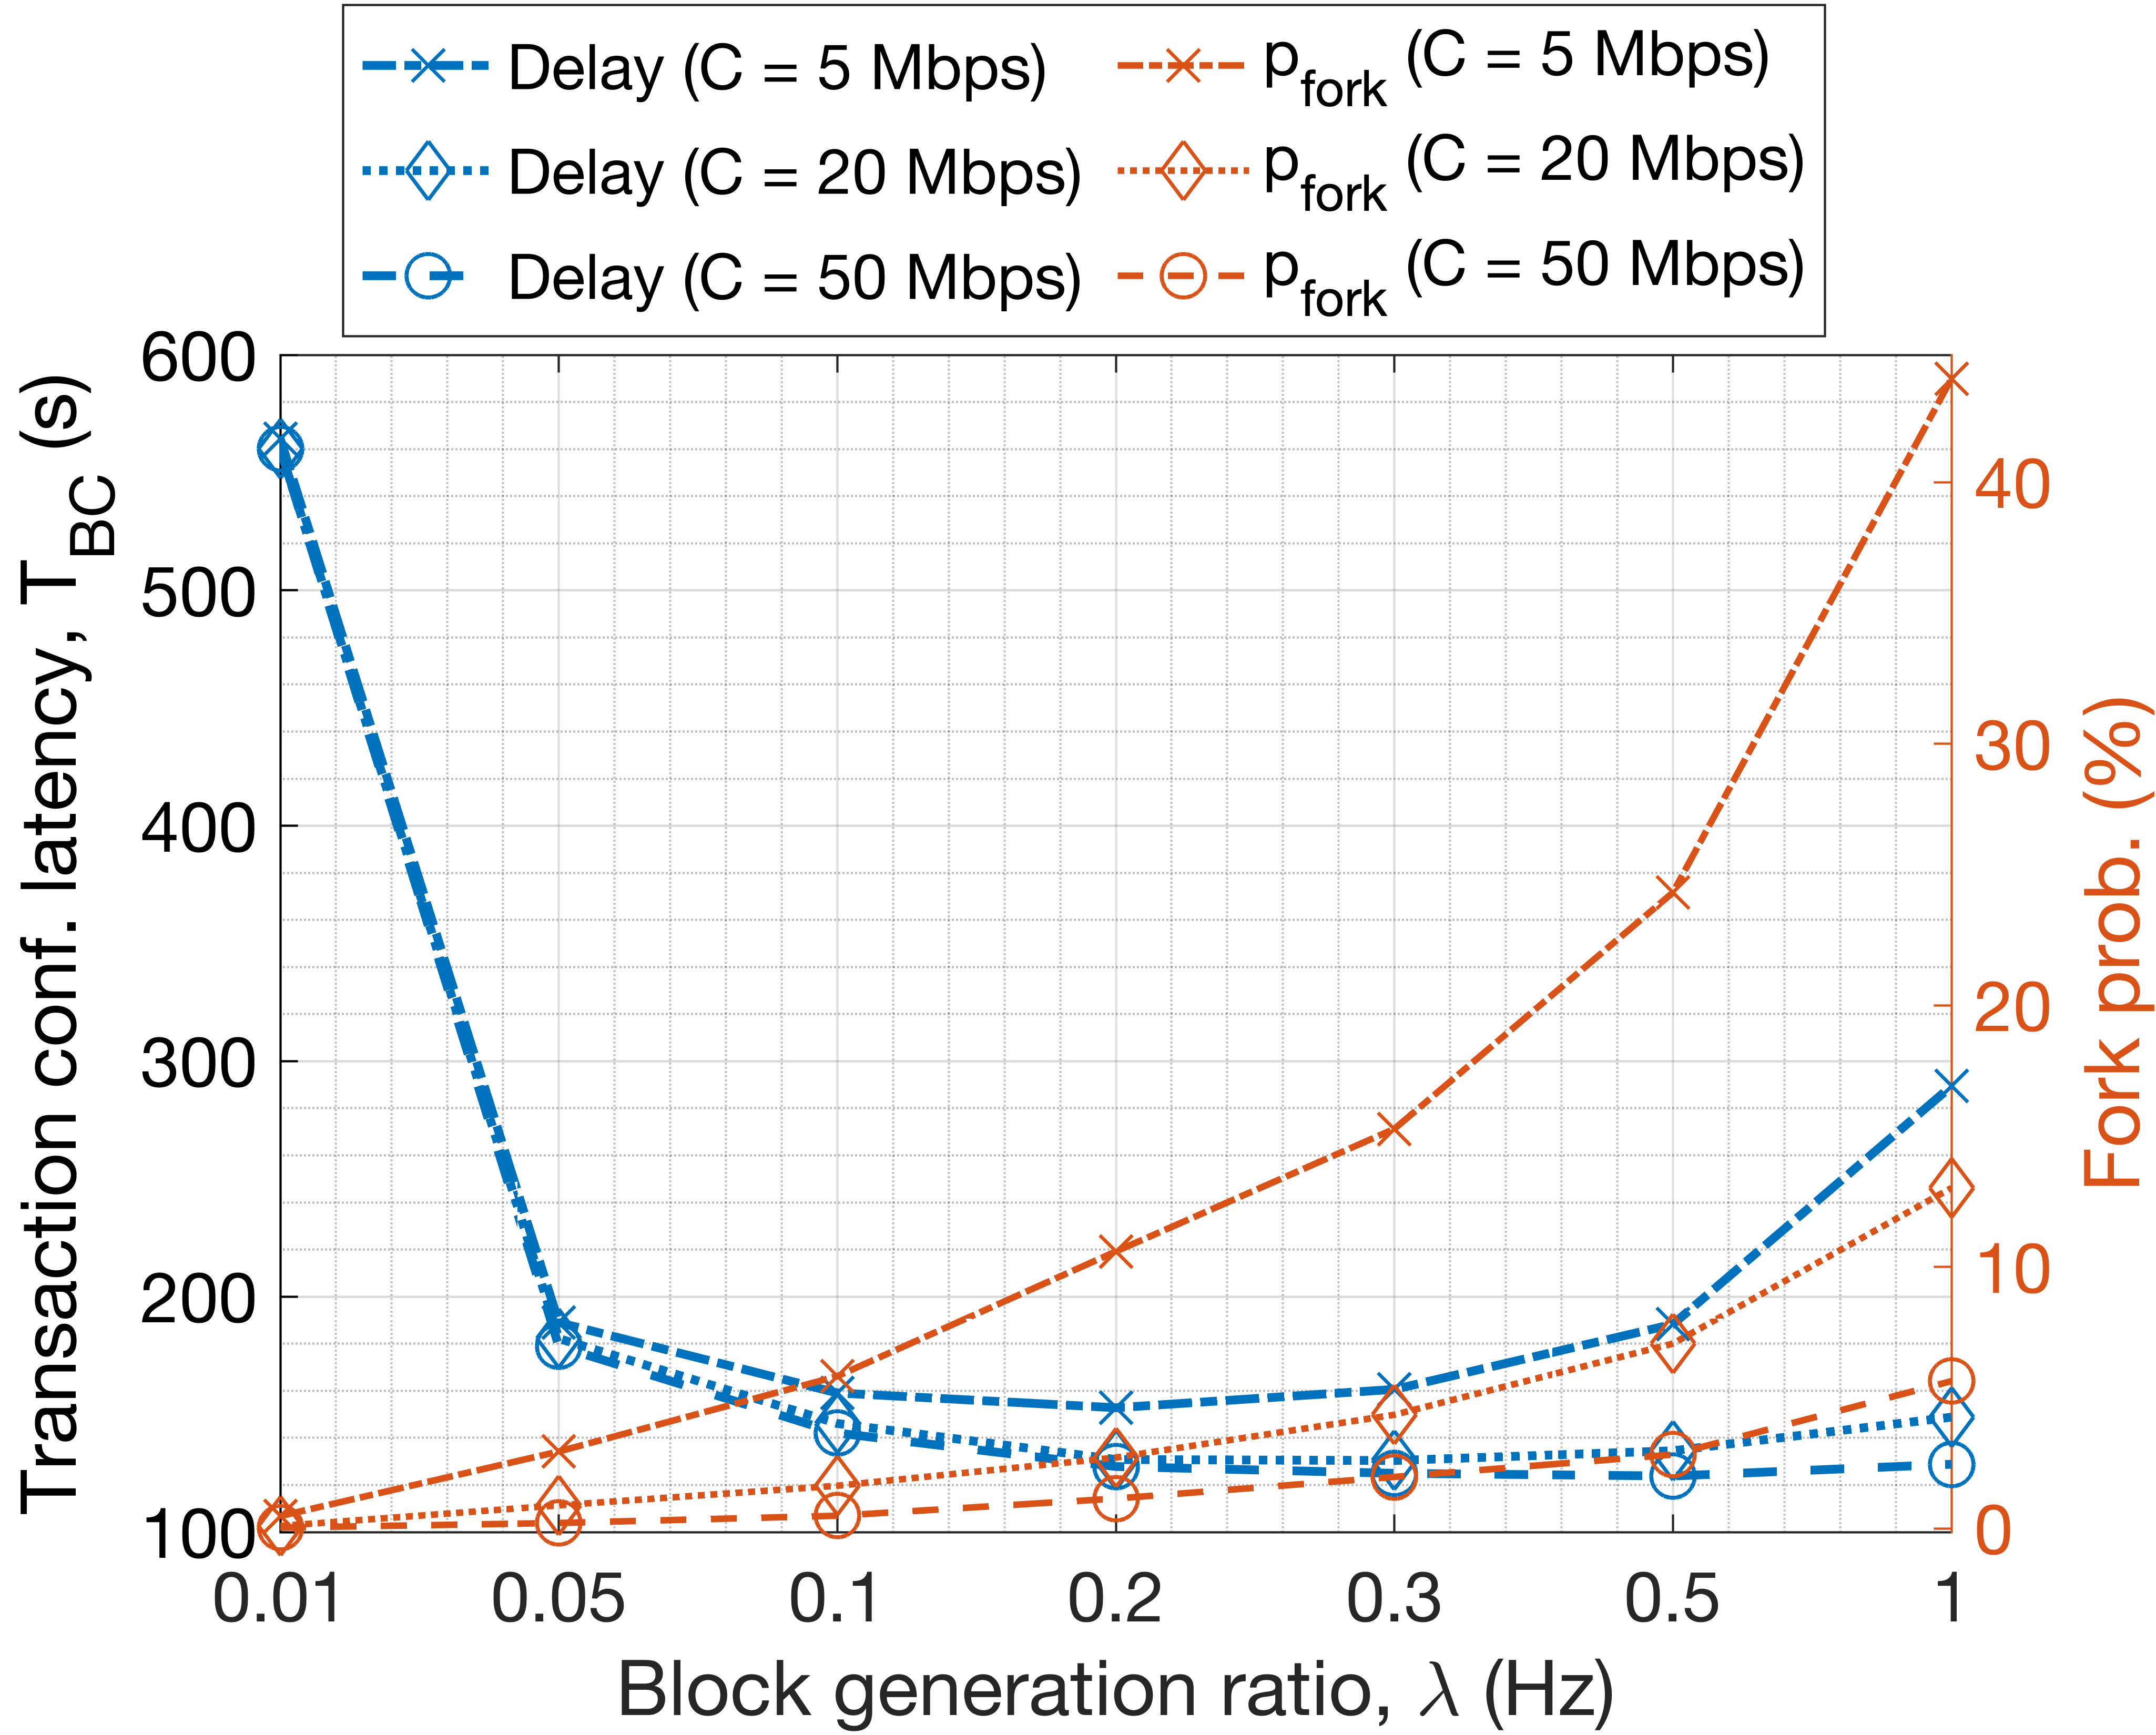
\includegraphics[width=.75\linewidth]{img/2_transaction_confirmation_delay_3.png}
	\caption{BC transaction confirmation latency ($\text{T}_\text{BC}$) and fork probability as a function of the block generation rate ($\lambda$).}
	\label{fig:4_transaction_confirmation_delay}
\end{figure}

Similar to the queue delay in Fig.~\ref{fig:bc_delay_mu}, the BC transaction confirmation latency has a concave shape, but now the effect of forks is exacerbated (especially for low capacities). The fact is that transactions involved in forks need to be re-included in the queue, which becomes critical as $\lambda$ increases. In contrast, high $C_\text{P2P}$ values allow mitigating the effect of forks and reducing the transaction confirmation latency. %Nevertheless, the capacity of the P2P network depends on the used underlying technology and, depending on the adopted solution, may not be high or suffer from congestion (e.g., P2P wireless links).

Finally, in Fig.~\ref{fig:5_delay_vs_block_size}, we plot the transaction confirmation latency as a function of the block size and the user arrivals rate. In particular, we show the results obtained by using $\lambda = \{0.05, 0.2, 1\}$~Hz with $C_\text{P2P} = 5$~Mbps.

\begin{figure}[ht!]
	\centering
	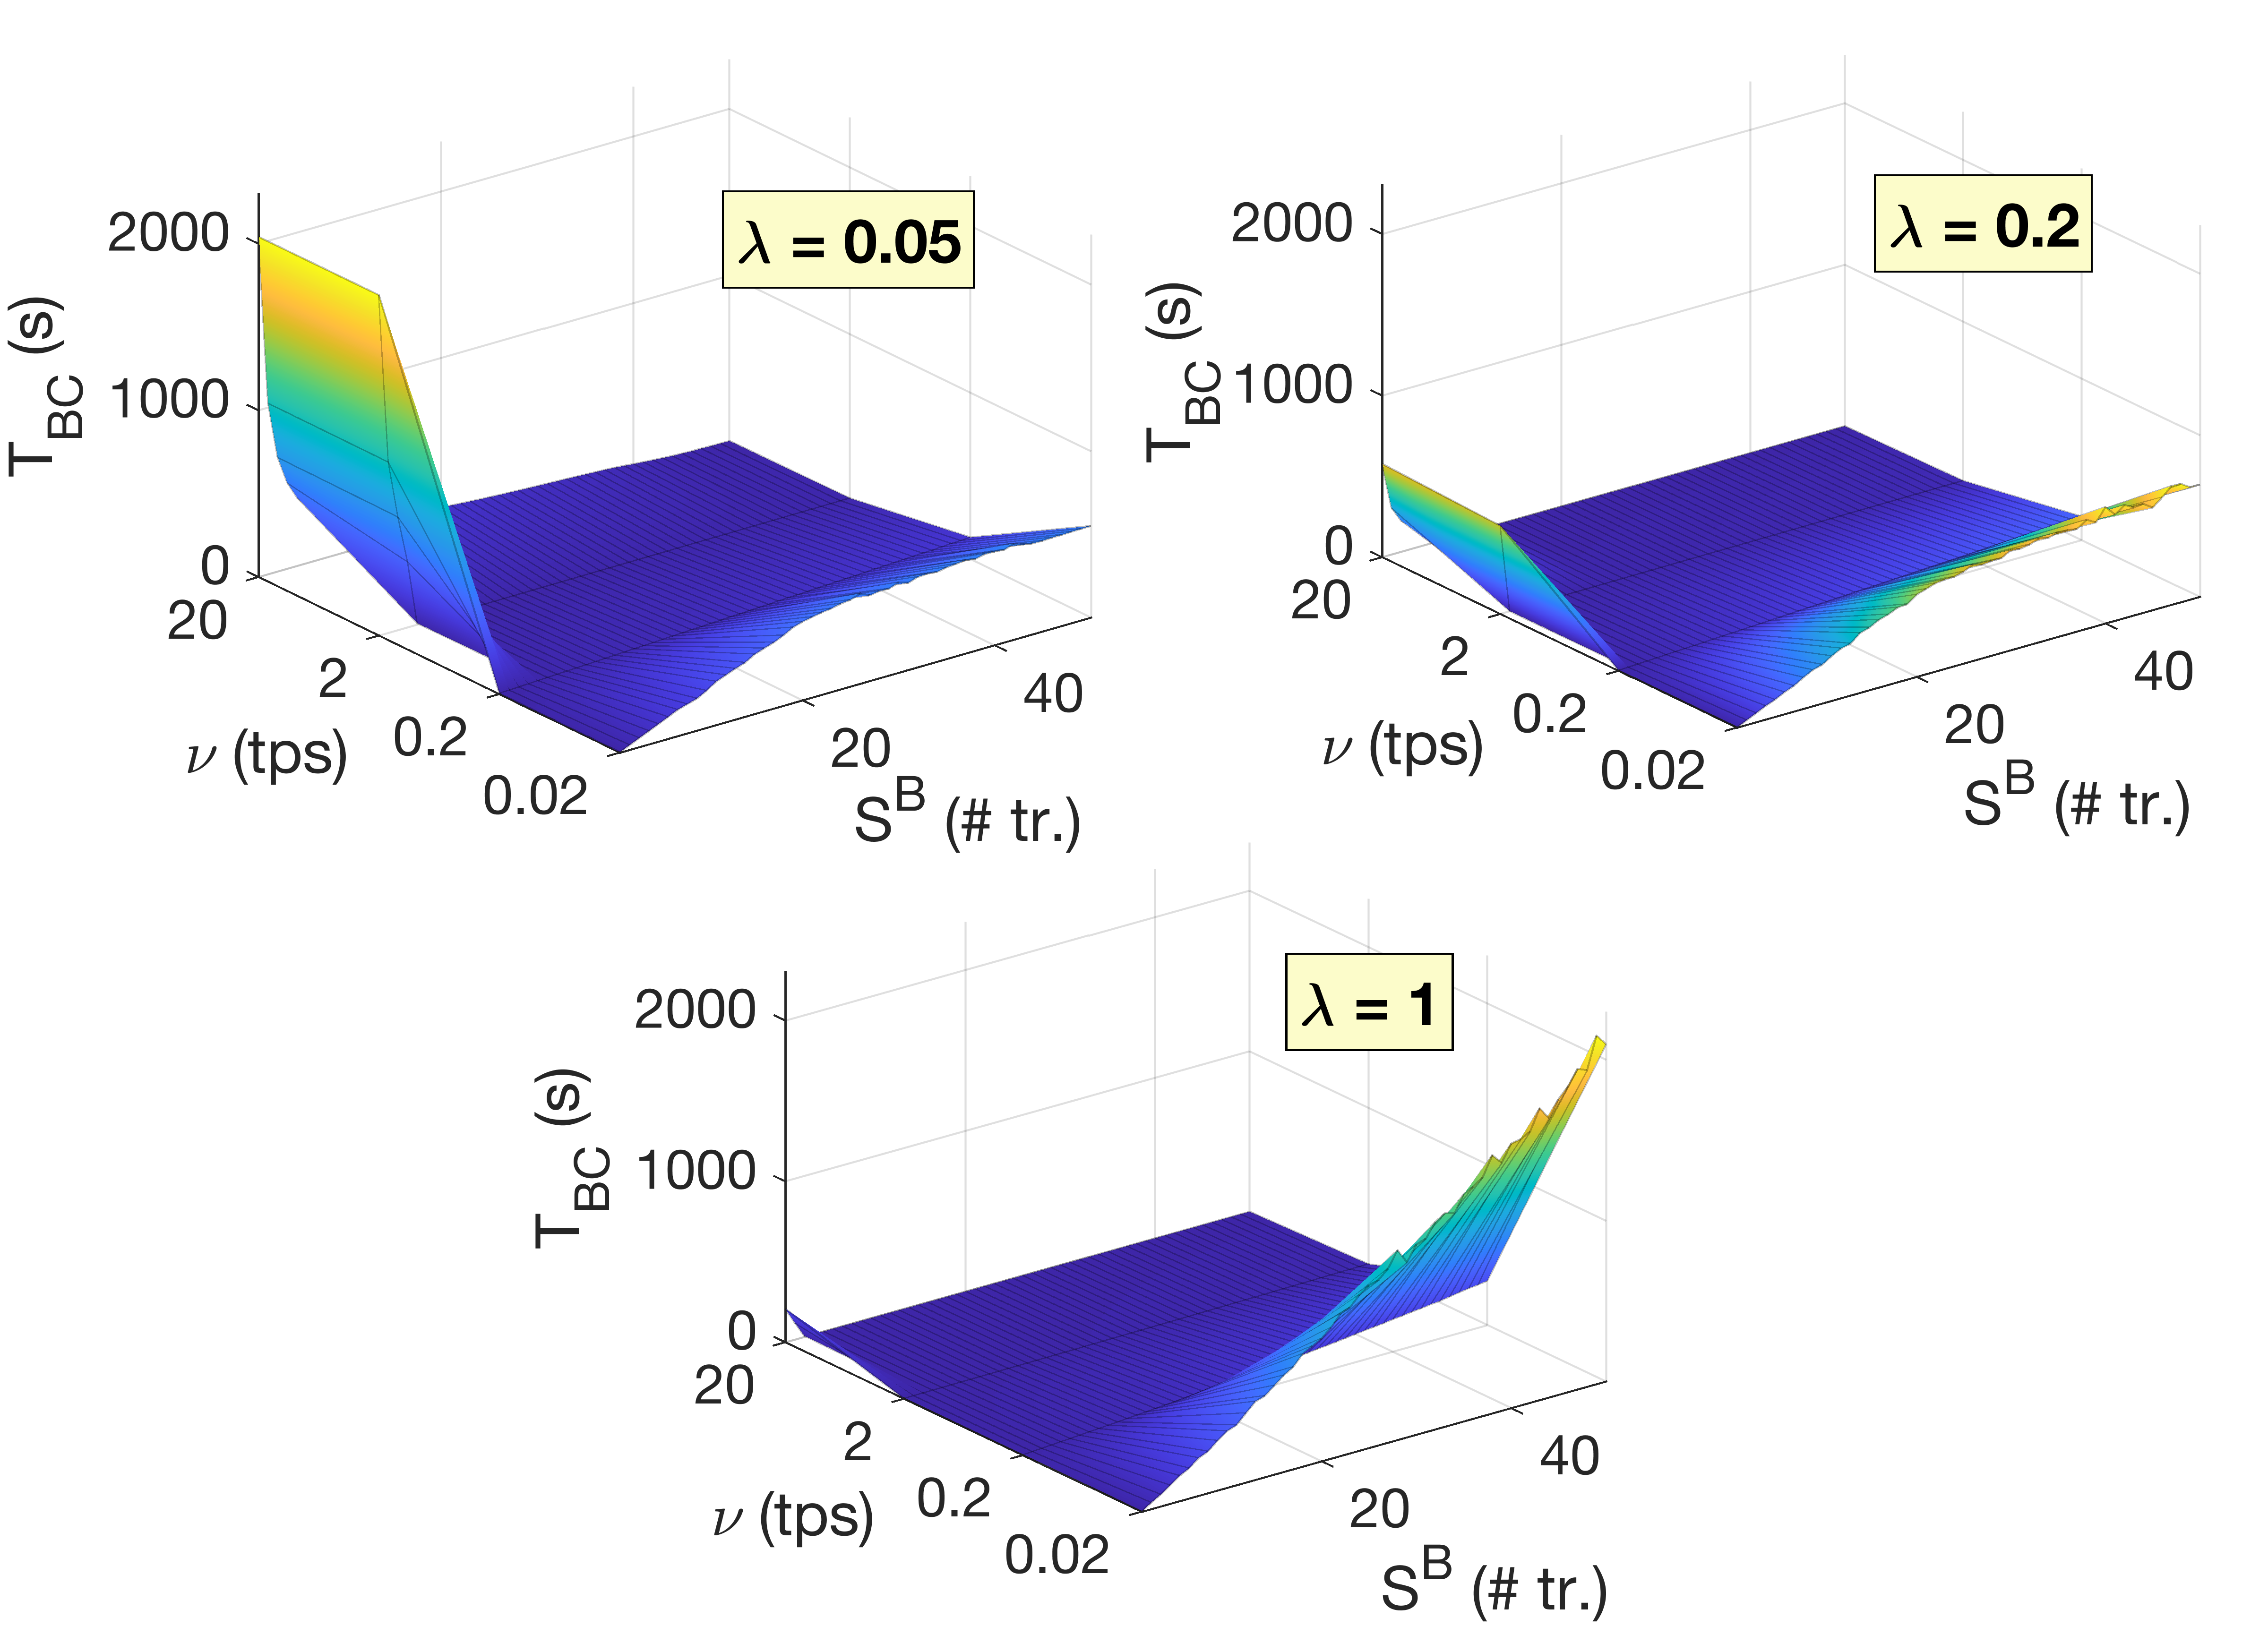
\includegraphics[width=\linewidth]{img/0_Tbc.png}
	\caption{BC transaction confirmation latency ($\text{T}_\text{BC}$) as a function of the block size ($S_\text{B}$) and the user arrivals rate ($\nu$), for $\lambda = \{0.05, 0.2, 1\}$ Hz.}
	\label{fig:5_delay_vs_block_size}
\end{figure}

Again, the relationship between the transaction confirmation latency and the block size behaves differently for different block generation ratios. For a low mining capacity (i.e., $\lambda=0.05$~Hz), using a small block size leads to very high delays, so that queue overflow occurs when heavy loads (e.g., $\nu=\{2,20\}$ transactions per second) cannot be absorbed. In contrast, for higher $\lambda$ values, the behavior varies and the trade-off between the block size and the fork probability becomes more evident. In any case, the proper election of the block size is essential for the sake of efficiency.

\subsection{s-FLchain vs a-FLchain}
\label{section:flchain_analysis}

To evaluate the s-FLchain and a-FLchain solutions, we use the well-known MNIST data set for federated image classification of handwritten digits~\cite{lecun1998mnist}. This data set contains data from 3,383 different users, including 341,873 training examples and 40,832 test samples for evaluation. Concerning the ML model, we have selected an out-of-the-box neural network (NN) with an input layer of 784 (one for each input data feature), a hidden layer of 256 neurons activated with the rectified linear unit function (ReLU), and an output layer with 10 neurons (one for each possible outcome). Model weights are optimized with SGD, based on the sparse categorical cross-entropy loss function.

In our evaluation, we split the data set into several partitions to focus on $K=\{10, 50, 100, 200\}$ random clients. Furthermore, to assess the impact of the asynchronous method, we adjust the block size in each FL round to consider smaller subsets of users, i.e., to accommodate data from $\Upsilon = \{10\%, 25\%, 50\%, 75\%\}$ of $K$ clients. Notice that the synchronized case corresponds to $\Upsilon = 100\%$ since all the considered clients' updates are included in a single block. The maximum waiting time $\tau$ is set to an arbitrarily high value to disregard its effect and focus on the block size only. Evaluation is carried out at $K_\text{eval} = 50$ different clients, which are independent from $K$ and are randomly sampled from the entire data set in each FL round. Furthermore, we use two variations of the MNIST data set, corresponding to independent and identically distributed (IID) and non-IID properties. Since clients typically have a rich number of samples for all the classes in the original data set~\cite{lu2020blockchain}, we break such an IIDness and restrict each client data set to 3 classes only (uniformly selected at random) in the non-IID case. In contrast, the IID case includes all the original samples in each client, containing data from up to 10 classes.

Fig.~\ref{fig:accuracy_loss_noniid} shows the mean evaluation accuracy exhibited by both sFLchain and aFLchain mechanisms, for both IID and non-IID settings during a fixed number of 200 FL rounds. Furthermore, we provide the baseline results obtained by a centralized method, which is trained using the entire MNIST data set (i.e., taking samples from all the clients). For comparison purposes, we have used the same hyper-parameters as for the federated settings. In addition, to avoid the high variability from the initial FL transitory phase, we plot the results from the last 50 iterations. 

\begin{figure}[ht!]
	\centering
	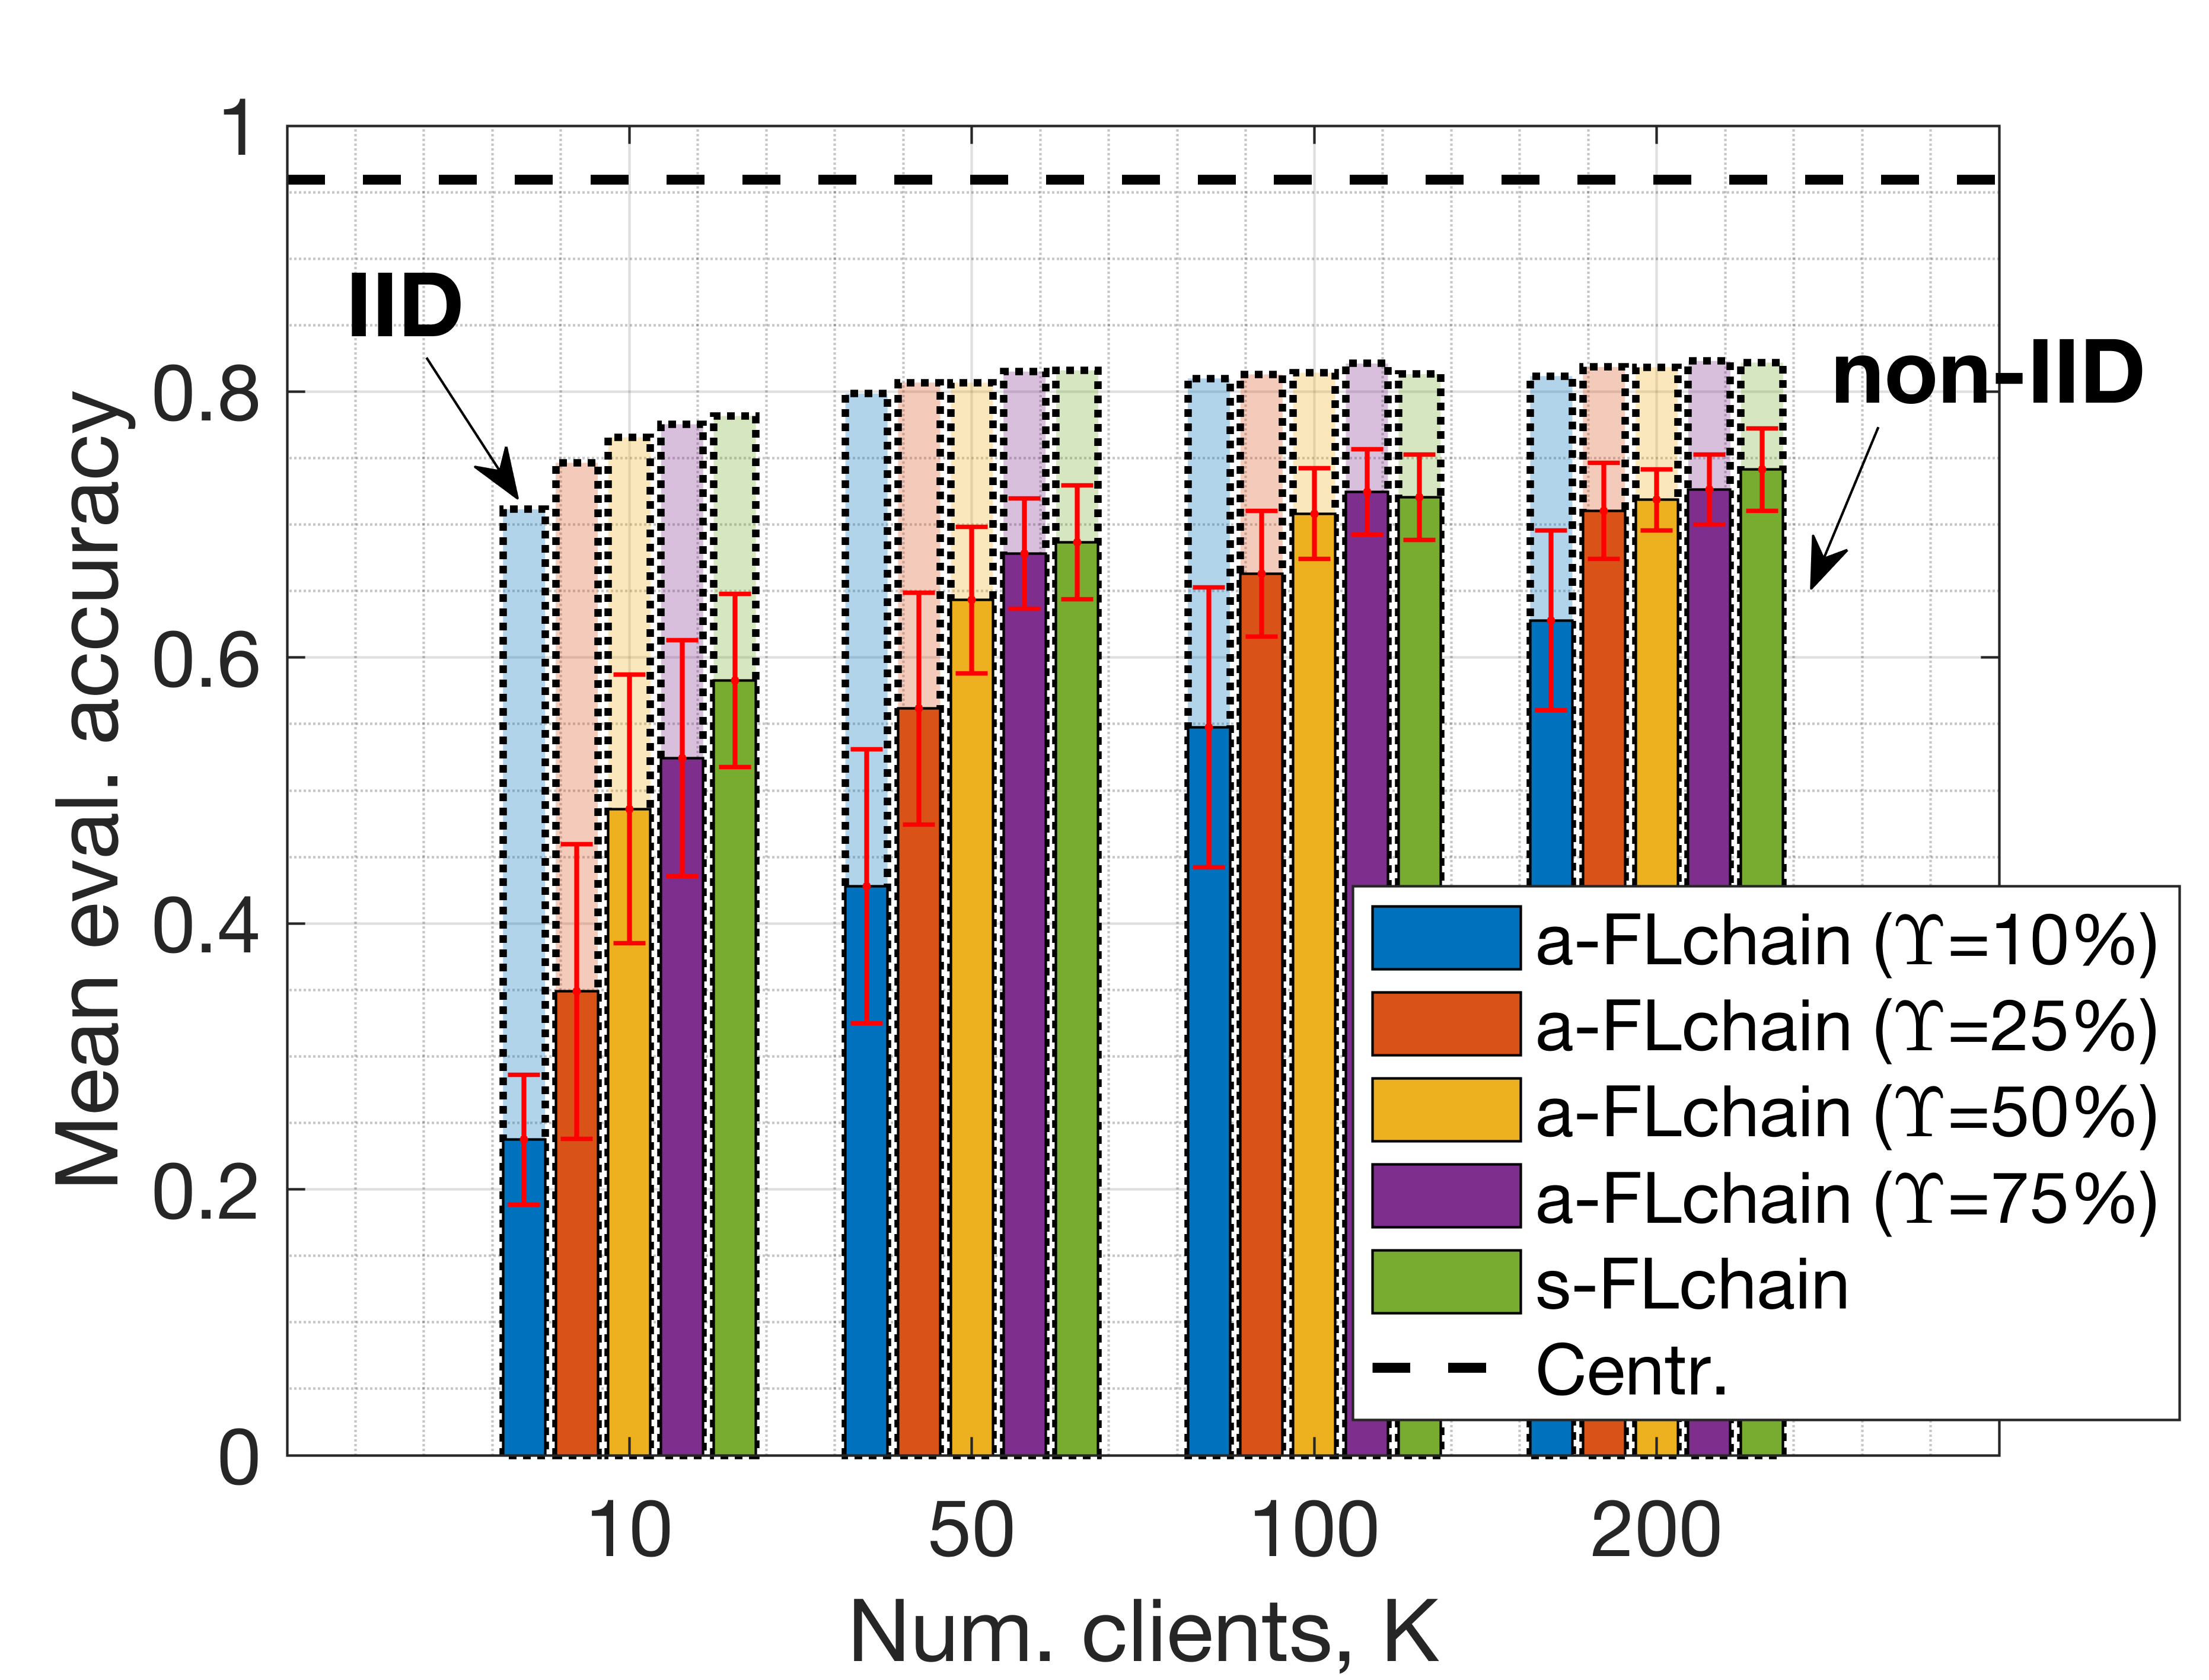
\includegraphics[width=0.75\columnwidth]{img/1_evaluation_accuracy.png}
	\caption{Mean evaluation accuracy obtained by s-FLchain and a-FLchain mechanisms on the IID (dashed bars) and non-IID (solid bars) versions of the MNIST data set, for a different number of clients $K$ and client sub-sampling percentages~$\Upsilon$. The centralized solution (black dashed line) is included for baseline performance. Only the last FL 50 iterations have been considered.}
	\label{fig:accuracy_loss_noniid}
\end{figure}

As shown, all the methods achieve a high accuracy for all the block sizes (represented by $\Upsilon$) in the IID setting, especially as $K$ increases. In this regard, we highlight the potential of the asynchronous method concerning the learning procedure since it allows achieving similar performance but using fewer data. When it comes to the non-IID setting, the performance of a-FLchain drops significantly when the number of participating clients in each iteration is low (for instance, for $K=10$ and $\Upsilon=10\%$). However, as more data is incorporated in each iteration, the performance improves.

\begin{figure*}[ht!]
	\centering
	\subfigure[]{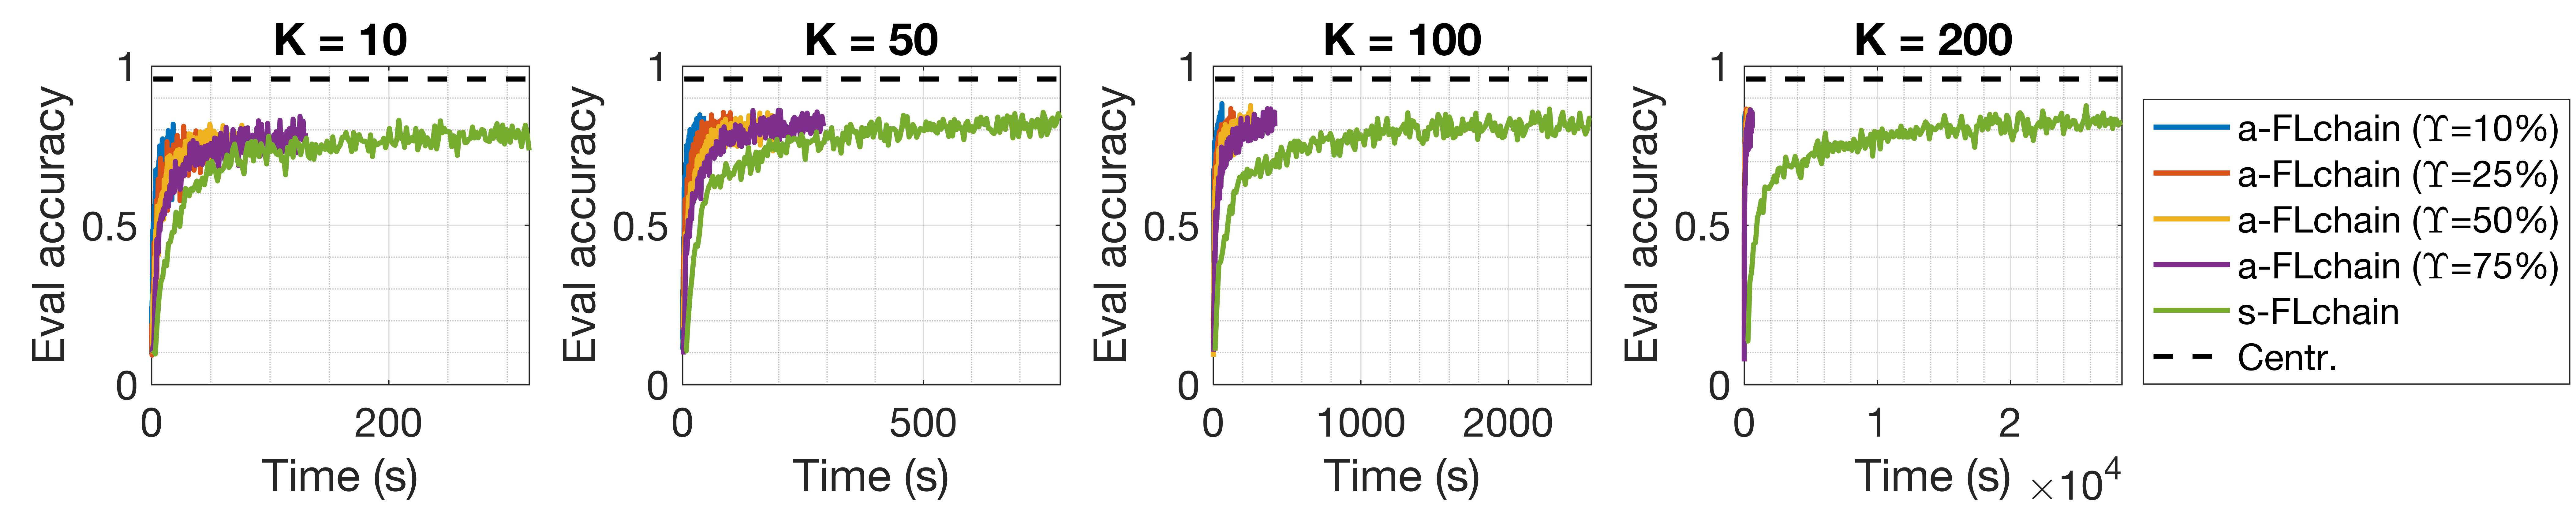
\includegraphics[width=.8\textwidth]{img/eval_accuracy_time_iid.png}\label{fig:eval_accuracy_iid}}
	\subfigure[]{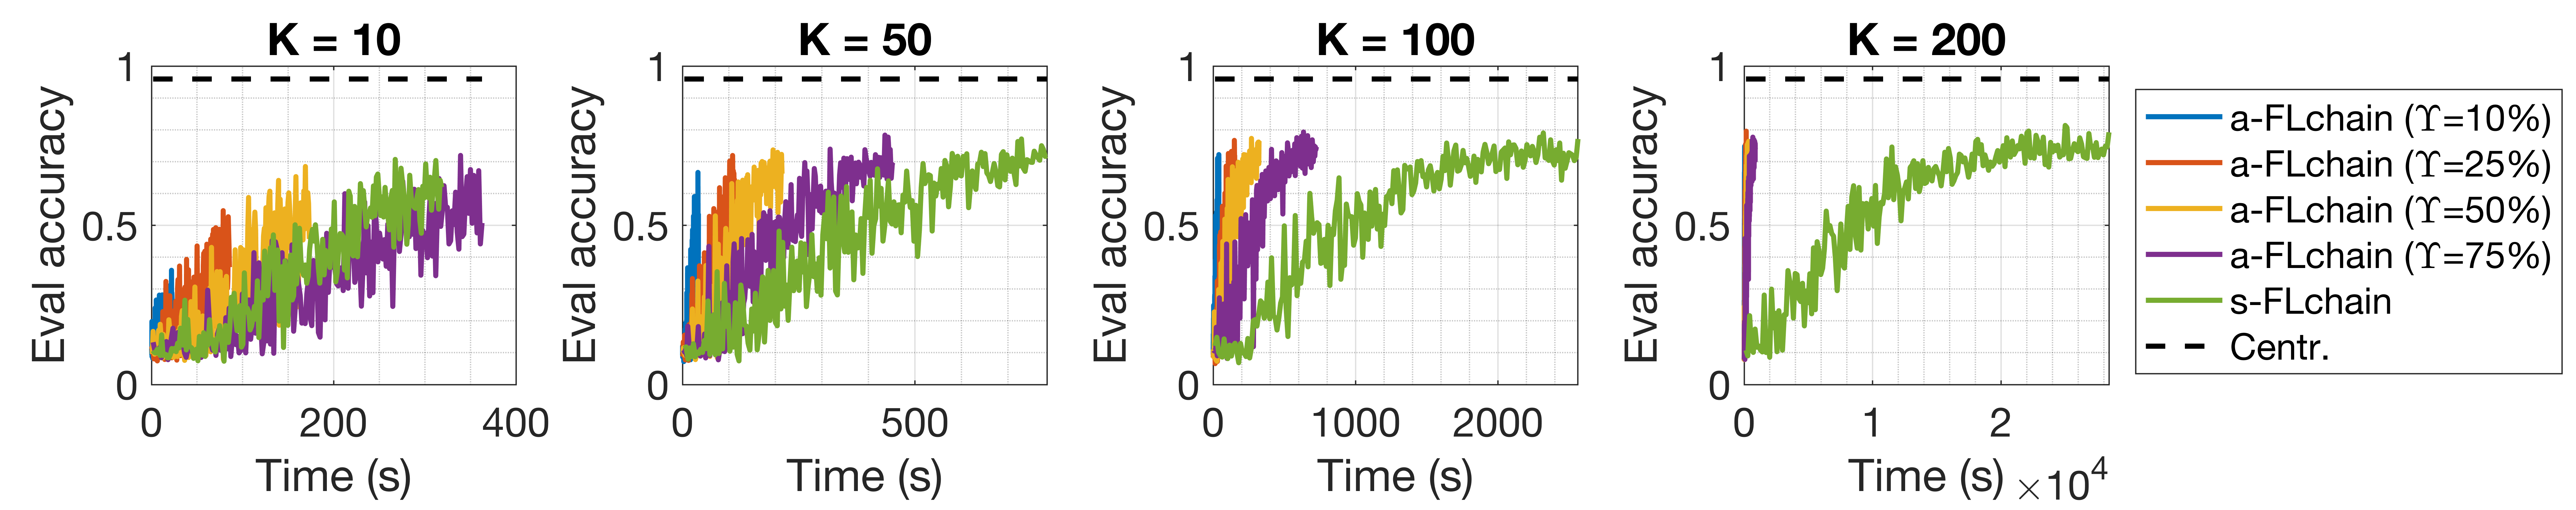
\includegraphics[width=.8\textwidth]{img/eval_accuracy_time.png}\label{fig:eval_accuracy_noniid}}
	\caption{Evaluation accuracy obtained by s-FLchain and a-FLchain on the MNIST data set, for different number of clients $K$ and client sub-sampling percentages~$\Upsilon$: (a) IID data, (b) non-IID data. The centralized solution (black dashed line) is included as a baseline.}
	\label{fig:temporal_evolution}
\end{figure*}

The s-FLchain method has shown better performance than a-FLchain, but let us now focus on the end-to-end latency and the temporal performance obtained throughout the considered 200 FL rounds. For that, we use the model provided in Section~\ref{section:delay_bc} to compute the iteration time in each of the applied mechanisms for each block size. Taking this into account, Fig.~\ref{fig:temporal_evolution} illustrates the evaluation accuracy and loss with respect to the time it takes to each method to complete the 200 rounds, for both IID (Fig.~\ref{fig:eval_accuracy_iid}) and non-IID (Fig.~\ref{fig:eval_accuracy_noniid}) settings. As done before, we evaluate the s-FLchain and a-FLchain using different numbers of users and block sizes.

From the temporal evolution of the accuracy, we observe that the asynchronous method may require a longer time to execute decentralized FL for short block sizes, i.e., for $K=10$ and $\Upsilon = 75\%$. This is mostly due to the incurred overhead, which leads to a high queuing time; a larger number of transactions need to wait in the pool before being served, including extra queuing time and time between blocks. In contrast, as the block size increases, a-FLchain becomes more efficient than s-FLchain in terms of iteration time but leads to similar accuracy (as shown before). Notice that the synchronized method requires a lot of time to include all the local updates to a single block. This is an important conclusion and suggests that a-FLchain is an appealing solution when dealing with large distributed data sets in FL. In those cases, and as shown later in Section~\ref{section:scalability_sflchain}, maintaining a strict synchronization among FL clients is counterproductive in terms of efficiency.

%%%%%%%%%%%%%%%%%%%%%%%%%%%%
%% Open directions
%%%%%%%%%%%%%%%%%%%%%%%%%%%%
\section{Ways Forward} %Open directions \textcolor{purple}{or challenges?}}
\label{section:open}

\subsection{Scalability issues with s-FLchain}
\label{section:scalability_sflchain}

One of the main results provided in this paper lies in the absence of scalability issues, shown instead by the PoW-based synchronous FL method (s-FLchain). In this regard, we have seen that, as the number of FL participants increases, the BC delay becomes higher, thus hampering the distributed learning procedure. To showcase the impact of the number of users and miners in s-FLchain in massive federated deployments, Fig.~\ref{fig:0_fork_probability} illustrates the fork probability in different settings. In particular, the fork probability increases with the number of users, which requires a higher block size to include all the synchronized transactions. Three different values of P2P link capacities are analyzed, as well as three different numbers of miners in the P2P network.

\begin{figure}[ht!]
	\centering
	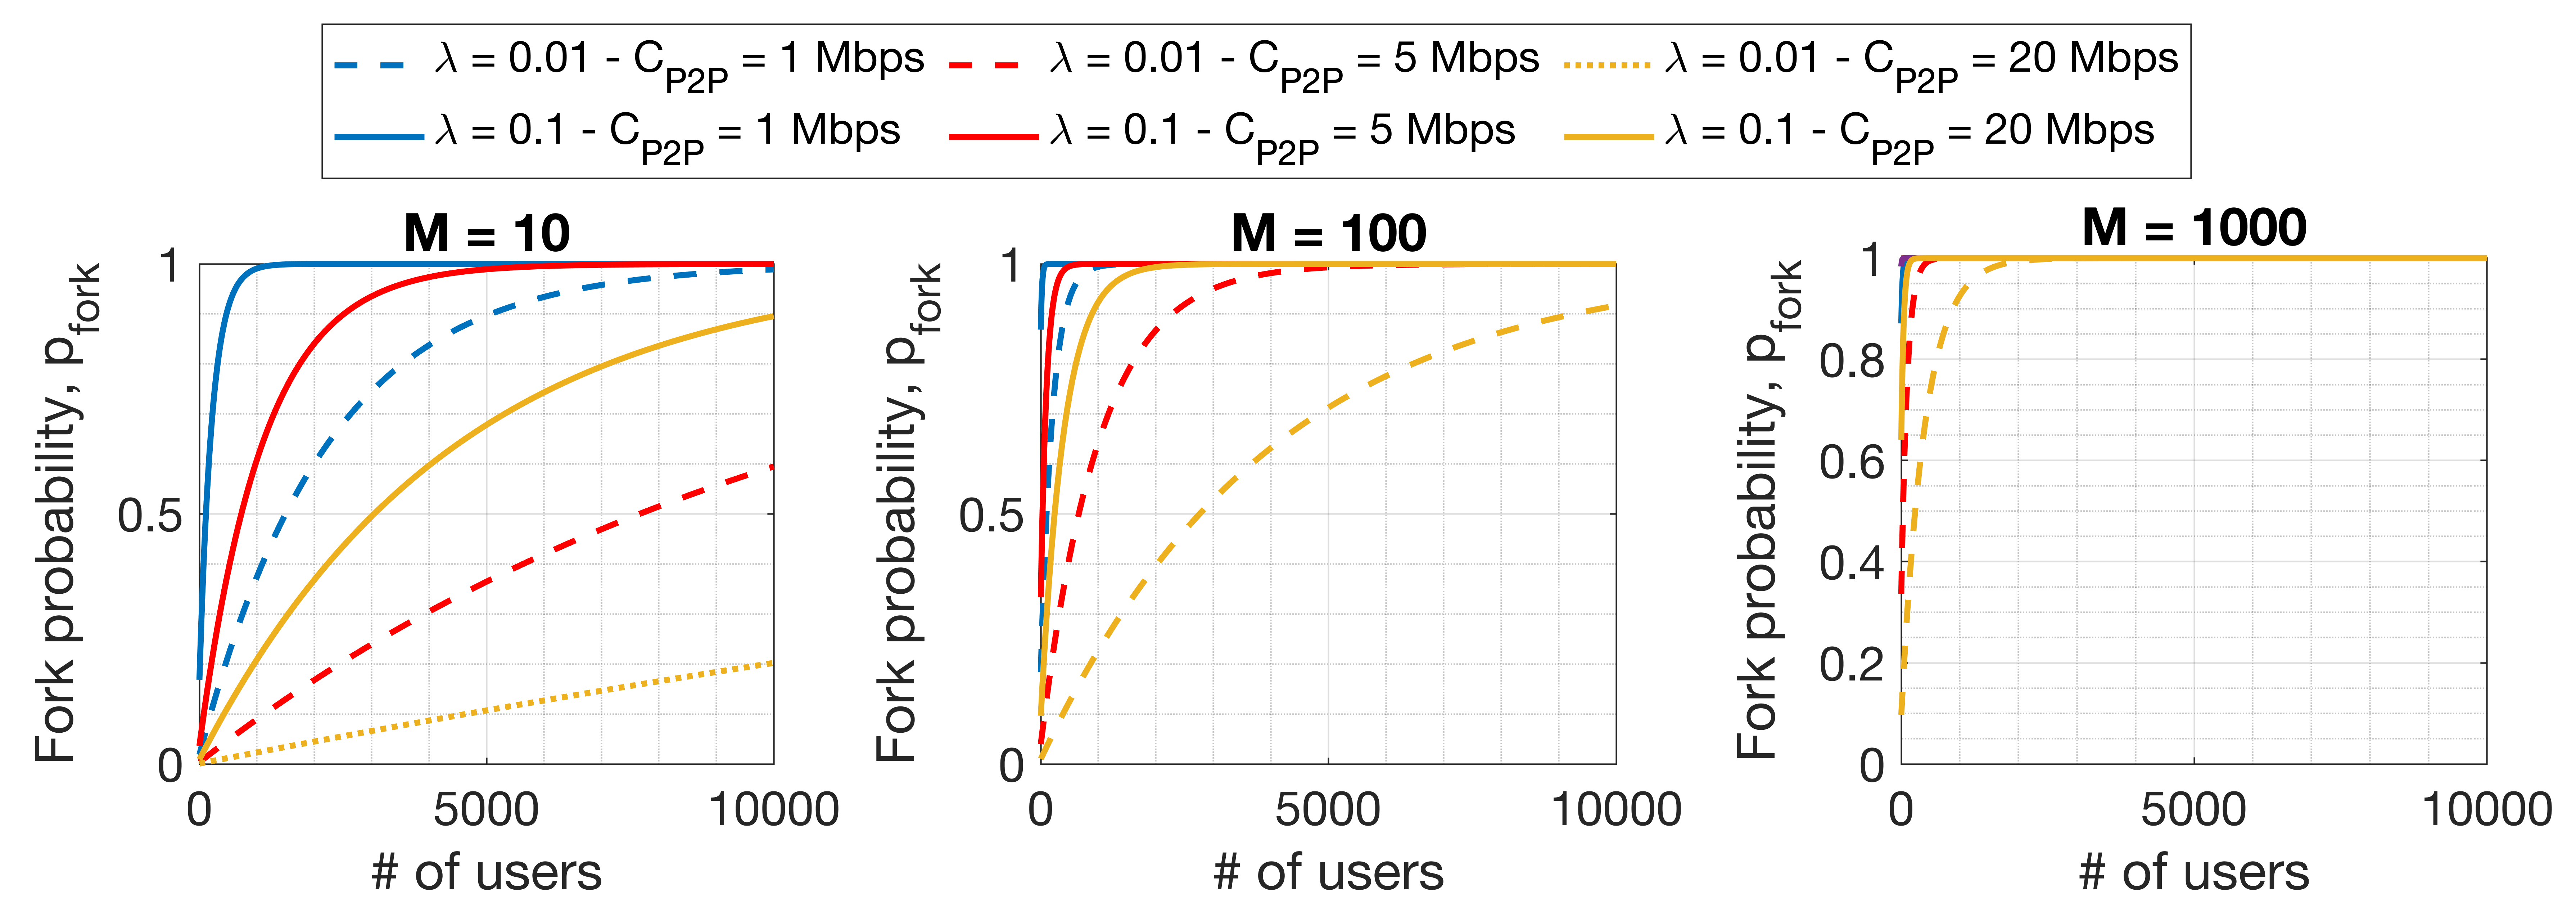
\includegraphics[width=1\linewidth]{img/0_fork_probability.png}
	\caption{Fork probability in PoW-based s-FLchain with respect to the number of users and miners.}
	\label{fig:0_fork_probability}
\end{figure}

As illustrated in the figure, the fork probability increases to very high values with the number of users, and this effect is amplified for bigger P2P networks with $M=100$ and $M=1000$ miners. In those situations, it is of utterance importance to provide high-capacity links for communication among miners. A high capacity allows to reduce the fork probability, thus significantly decreasing the FL round time. In more reduced deployments (with $M=10$ miners and up to $K=200$ users), a high P2P capacity allows the s-FLchain to improve efficiency, therefore providing shorter iteration times, even lower than for certain a-FLchain settings (which may incur into more overheads). To illustrate this, Fig.~\ref{fig:fl_round_time_more_capacity} shows the FL round time obtained by each solution, as done in Section~\ref{section:flchain_analysis}, but for $C_\text{P2P} = 25$~Mbps, instead of the previously considered $C_\text{P2P} = 5$~Mbps. As shown in Fig.~\ref{fig:fl_round_time_more_capacity}, short FL round times (maximum of 3~s) are obtained, even for large block sizes (e.g., $K=200$ users). In addition, we observe that s-FLchain improves a-FLchain in certain settings, i.e., for $K=\{50,100,200\}$ and $\Upsilon=\{50,75\}\%$. The reason is that the provided high capacity allows mining big blocks very fast in the synchronous setting, thus overcoming the effect of forks. In contrast, in a-FLchain, the idle periods entail a significant overhead in terms of FL round time. 

\begin{figure}[ht!]
	\centering
	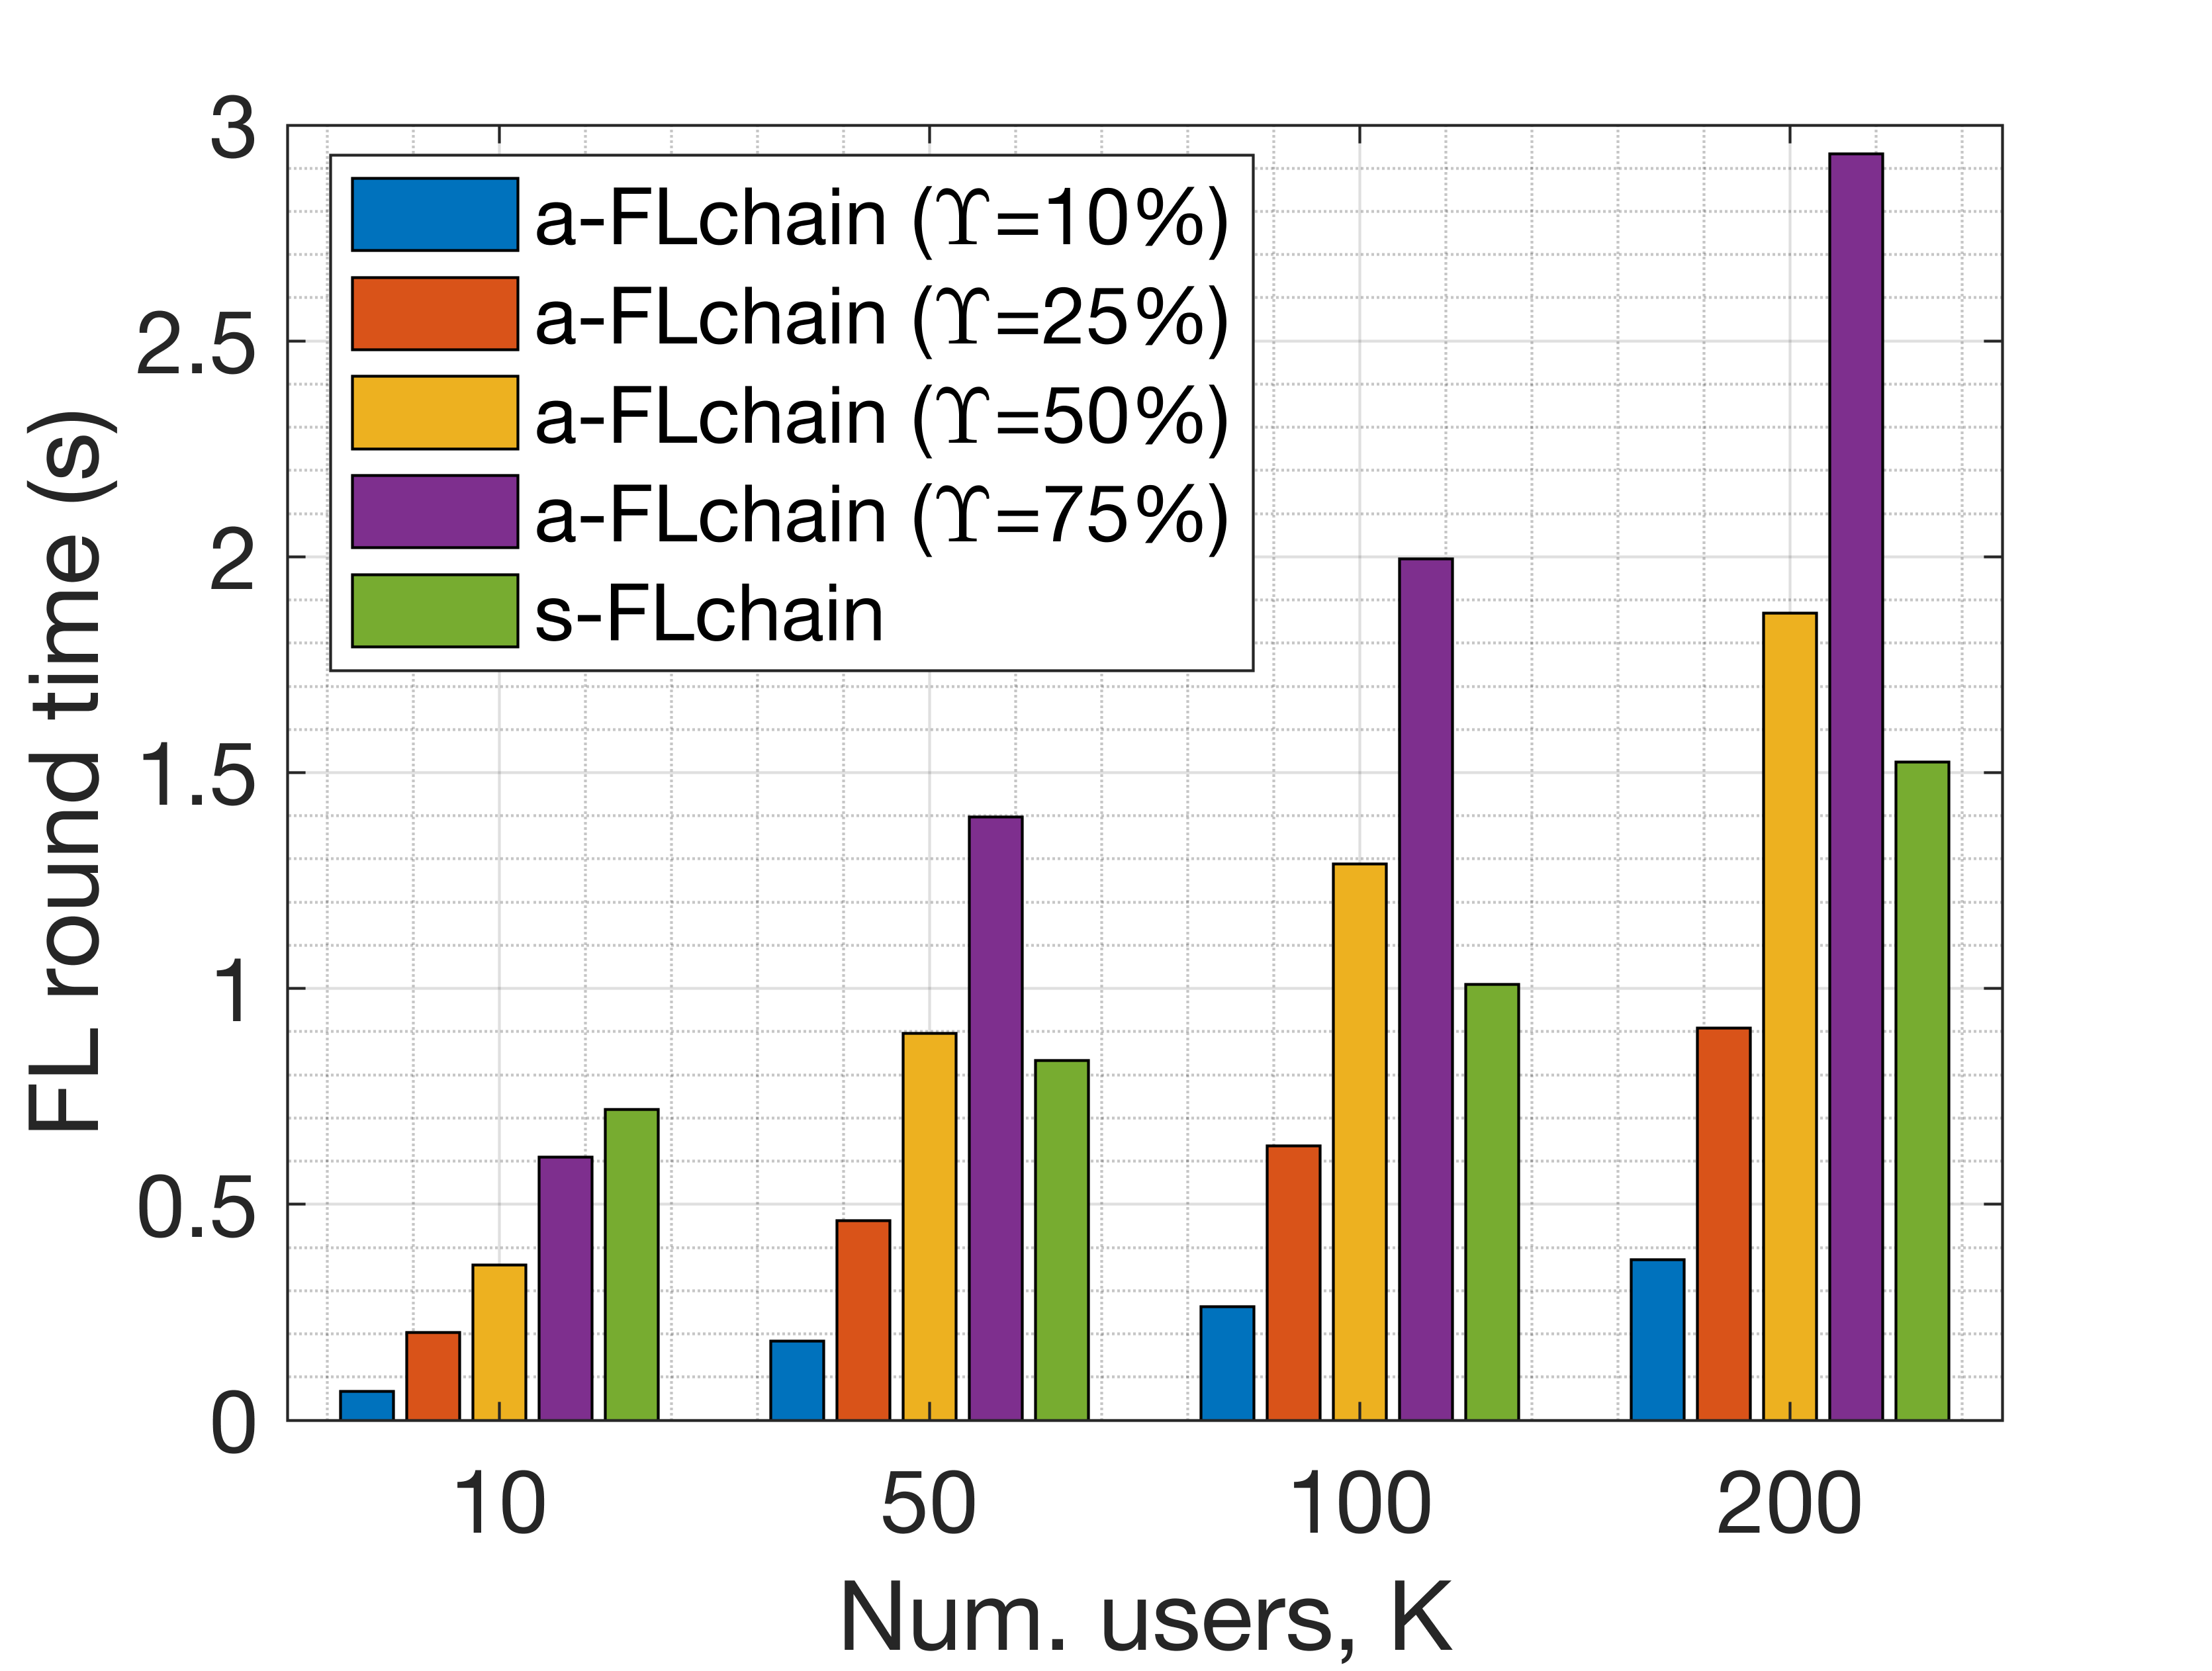
\includegraphics[width=.7\linewidth]{img/2_fl_round_time_more_capacity.png}
	\caption{Effect of increasing the capacity between peer nodes ($C_\text{P2P}=25$ Mbps) on the FL round time, for different number of clients $K$ and client sub-sampling percentages~$\Upsilon$.}
	\label{fig:fl_round_time_more_capacity}
\end{figure}

An important conclusion is that the P2P capacity has a strong impact on the performance of a BC. Thus, the proper analysis of the behavior of BCs running over realistic bandwidth-constrained networks becomes of topical importance. In~\cite{wilhelmi2021performance}, for instance, wireless BC networks were analyzed for contention-based communication schemes (e.g., Wi-Fi). Concerning FLchain, we have already shown that the network characteristics and the ongoing traffic have a huge impact on the federated optimization process. In this regard, future contributions are expected in the \emph{communications for FL} field~\cite{chen2020wireless}.

%A high capacity leads to more robust and reliable information exchanges, while low capacity may lead to extra delays and energy consumption (due to the effect of forks). 

\subsection{Open aspects in a-FLchain}
\label{section:open_aspects_aflchain}

The FLchain solution naturally leads to an asynchronous setting, whereby disordered updates may lead to differences in training FL models. In asynchronous FL, aggregation is done in parallel to the reception of local updates, so that every time a local update is available, a global model update is provided (see Fig.~\ref{fig:sync_vs_async_diagram} in Section~\ref{sec:introduction}).

Although the asynchronous setting has been shown to provide good performance on SGD optimizations through experimental results~\cite{xie2019asynchronous, sprague2018asynchronous, chen2020asynchronous}, it also entails several challenges, especially related to device and data heterogeneity~\cite{xu2021asynchronous}. When devices have diverse capabilities (e.g., computation, communication, availability), the asynchronous FL optimization may fail and lead to biased global models~\cite{chen2020asynchronous}, influenced by the most participating nodes (i.e., nodes with better capabilities). To address the issues arising from devices heterogeneity, some proposals include the usage of semi-asynchronous settings and weighted averaging. Assigning higher weights to best-performing nodes works particularly fine for IID datasets. Regarding data heterogeneity, clustering by similarity (e.g., localized training, personalized training) has been shown as an appealing solution, but other methods like transfer learning or meta-learning are gaining attention. %Notice that, as shown in~\cite{chen2020asynchronous}, the asynchronous setting is more susceptible to failure when data is highly heterogeneous, i.e., for non-IID settings.

Another implication of the asynchronous FL setting is that global updates may include data from clients using outdated models, which contributes to the instability of the system. To address inconsistencies among client models, a widely accepted approach is to quantify the model differences in each FL iteration. For instance, \cite{xie2019asynchronous} proposes a staleness coefficient to guarantee convergence and ensure stability. Similarly, a decay coefficient to balance past and new data is used in~\cite{chen2020asynchronous}. Other solutions may include mechanisms like using sliding windows to compute global updates, or assessing the quality of individual local updates before doing aggregation. 

\subsection{Architectural considerations in FLchain}
\label{section:architectural_considerations}

%Moreover, FLchain has been envisioned to run over multiple architectural solutions, thus being empowered by paradigms like edge computing~\cite{majeed2019flchain}, fog computing~\cite{qu2020decentralized}, or peer-to-peer (P2P) communications~\cite{kim2019blockchained, ma2021federated}. For a more comprehensive view on the potential uses cases of FLchain for 5G and beyond, refer to the work in~\cite{lu2020blockchain2}. 

Adopting blockchain for FL allows removing the figure of a central server authority that orchestrates the learning procedure and aggregates data. However, in the FLchain setting, several architectural aspects remain open and may arise concerns on learning accuracy, overall latency, and energy consumption.

In this paper, we have considered that FL model aggregation is performed at clients locally, so that they retrieve all the local updates from the latest valid block, generate the global model accordingly, and start computing a new local update. However, aggregation can be potentially done by edge servers, which may also act as miners. The edge offloading solution entails adding a certain hierarchy to the system, but promises performance improvements and addressing issues related to devices heterogeneity.

Similarly, when it comes to the BC operation, the FL iteration time is affected by the location of miners and their corresponding interactions with FL users for receiving and propagating transactions. One possibility is locating miners in the cloud, which turns out to be a feasible solution due to the easiness of deployment. Alternatively, operators could provide mining capabilities to their base stations via mobile edge computing (MEC), thus significantly accelerating the BC operation for securing transactions and blocks. Finally, a more revolutionary vision consists of maintaining fully decentralized networks of miners, to which clients can communicate via D2D links. With this, any interested party (e.g., a personal handheld device) can become a miner and provide support to maintain the BC. However, due to the heterogeneous computation capabilities and availability of regular devices, such a solution would entail a set of unprecedented challenges.

\subsection{Blockchain consensus}
\label{section:consensus}
To maintain a distributed ledger, miners and peer nodes collaborate following a given consensus mechanism. In this paper, we have focused on a model and performance of public, PoW-based FLchain mechanisms. Nevertheless, other consensus strategies can be leveraged to fulfill multiple purposes (see Table~\ref{tab:consensus}).\footnote{Note that the provided throughput and latency values are approximated and serve as an average indicator, given the rich set of implementations of the different algorithms providing various performances.} In this regard, an important aspect to be taken into consideration consists in the access privileges of the BC, i.e. whether it is public (permissionless) or private (permissioned). This is briefly discussed in what follows:
\begin{itemize}
	\item \textbf{Permissionless:} governance is public, so any interested party can participate. A public BC allows for high transparency and low synchronization but may lead to a low capacity in terms of transactions per second.
	\item \textbf{Permissioned:} governance is private or by a consortium, so only authorized peer nodes can participate. Permissioned BCs provide higher throughput than permissionless ones.
\end{itemize}

 %For more details regarding BC consensus mechanisms, refer to the work in~\cite{nguyen2018survey}.

\begin{table}[ht!]
	\caption{Overview of some of the most popular consensus protocols for BC.}
	\label{tab:consensus}
	\resizebox{\columnwidth}{!}{%
		\begin{tabular}{|l|c|c|c|c|}
			\hline
			\multicolumn{1}{|c|}{\textbf{\begin{tabular}[c]{@{}c@{}}Consensus Protocol\end{tabular}}} & \textbf{Ref.} & \textbf{Type} & \textbf{Throughput} & \textbf{Latency} \\ \hline
			\begin{tabular}[c]{@{}l@{}}Proof-of-Work (PoW)\end{tabular} & \cite{nakamoto2019bitcoin} & Public & $<10$ tps & ~10 min \\ \hline
			\begin{tabular}[c]{@{}l@{}}Proof-of-Stake (PoS)\end{tabular} & \cite{saleh2021blockchain} & Public/Private & 10-1,000 tps & $<1$ min \\ \hline
			\begin{tabular}[c]{@{}l@{}}Proof of Reputation \\ (PoR)\end{tabular} & \cite{gai2018proof} & Private & ~1,000 tps & 10-30 s \\ \hline
			\begin{tabular}[c]{@{}l@{}}Practical Byzantine \\ Fault Tolerance (PBFT)\end{tabular} & \cite{castro1999practical} & Public & 100-10,000 tps & $<1$ min \\ \hline
			\begin{tabular}[c]{@{}l@{}}Ripple Protocol \\ Consensus Algorithm\\ (RPCA)\end{tabular} & \cite{schwartz2014ripple} & Private & 1,000-100,000 tps & $<1$ s \\ \hline
		\end{tabular}%
	}
\end{table}

%\textcolor{red}{An important conclusion that can be provided is that fully distributed consensus mechanisms hamper the FL procedure by incurring into excessive delays in dense scenarios (with multiple miners and intense client updates). So, mechanisms like PoW cannot be directly applied to (near)real-time problems because they require a certain amount of time (from tens of seconds to minutes) to generate stable consensus (in~\cite{kim2019blockchained}), the learning completion time is of the order of 1000 seconds in very small scenarios (with 10 miners and 10 clients). Therefore, we can propose other hierarchical consensus mechanisms that eliminate the existence of forks.}

Finally, another uncovered aspect lies in the incentives provided for participating in the consensus, whereby peer nodes obtain revenues for carrying out operations like mining. Since BC participants may act as rational players, this opens the door to various sets of strategies and malicious behaviors. This is where game theory comes into play and serves as a powerful tool to analyze strategies resulting from different consensus protocols, or to define the appropriate incentive mechanisms to avoid undesired behaviors (e.g., selfishness, attacks). Indeed, assigning rewards to miners and clients has been shown to leverage the FLchain scheme to obtain better results~\cite{toyoda2019mechanism}. A comprehensive survey on game theory in BC can be found in~\cite{liu2019survey}. 

%The performance of a BC in terms of throughput, overhead, and transaction confirmation latency is affected by the following important aspects:
%\begin{itemize}
%    \item The adopted consensus mechanism whereby miners mine blocks (e.g., Proof-of-Work, Proof-of-Stake) and the mining difficulty, which determines the mining delay. Moreover, in decentralized types of BCs, forks may occur as a result of simultaneous mined blocks.
%
%    \item The size of the blocks and transactions to be propagated over the blockchain. A maximum block size is defined to avoid the network being overloaded with arbitrarily large blocks.
%
%    \item The size of the P2P network running the blockchain, as well as the communication technology used by the P2P network to exchange information. These characteristics strongly affect the total block propagation time and may potentially lead to synchronization issues.
%
%    \item The attitude of peer nodes, including malicious behaviors that may affect the performance of the BC. For instance, a malicious miner may intentionally retain transactions to increase its probability of mining the next block.
%\end{itemize}

%%%%%%%%%%%%%%%%%%%%%%%%%%%%
%% CONCLUSIONS
%%%%%%%%%%%%%%%%%%%%%%%%%%%%
\section{Conclusions}
\label{section:conclusions}
This paper has addressed an emerging topic regarding distributed federated optimization and has proposed the usage of BC technology to realize it in a secure, transparent, and reliable manner. To assess the feasibility of this BC-enabled solution, an end-to-end latency framework has been developed, including a novel queuing model suitable to BC technology. Based on this framework, synchronous and asynchronous methods (s-FLchain and a-FLchain) are evaluated in terms of accuracy and latency. While the synchronous version allows obtaining a high accuracy for both IID and non-IID data sets, its iteration time becomes very high for a large number of users. This prevents the adoption of this kind of mechanisms in massive deployments, thus lacking scalability. In contrast, the asynchronous FL optimization solution provides good accuracy results while keeping the overhead low, depending on the number of local updates included in each iteration via BC. Future research directions include innovative mechanisms and architectural solutions for FLchain, able to address the challenges raised by either BC implementations (e.g., capacity, latency) or the device and data heterogeneity in asynchronous training.

%Synchronized FLchain applications are narrowed to applications with a small number of federated devices.


% if have a single appendix:
%\appendix[Proof of the Zonklar Equations]
% or
%\appendix  % for no appendix heading
% do not use \section anymore after \appendix, only \section*
% is possibly needed

% use appendices with more than one appendix
% then use \section to start each appendix
% you must declare a \section before using any
% \subsection or using \label (\appendices by itself
% starts a section numbered zero.)
%


%\appendices
%\section{Proof of the First Zonklar Equation}
%Appendix one text goes here.
%
%% you can choose not to have a title for an appendix
%% if you want by leaving the argument blank
%\section{}
%Appendix two text goes here.


% use section* for acknowledgment
\ifCLASSOPTIONcompsoc
  % The Computer Society usually uses the plural form
  \section*{Acknowledgments}
\else
  % regular IEEE prefers the singular form
  \section*{Acknowledgment}
\fi


This work was funded by the IN CERCA grant from the Secretaria d'Universitats i Recerca del departament d'Empresa i Coneixement de la Generalitat de Catalunya, and partially from the Spanish grant PID2020-113832RB-C22 (ORIGIN) and the European Union’s Horizon 2020 research and innovation programme under Grant Agreement No. 953775 (GREENEDGE). 

% Can use something like this to put references on a page
% by themselves when using endfloat and the captionsoff option.
\ifCLASSOPTIONcaptionsoff
  \newpage
\fi

% trigger a \newpage just before the given reference
% number - used to balance the columns on the last page
% adjust value as needed - may need to be readjusted if
% the document is modified later
%\IEEEtriggeratref{8}
% The "triggered" command can be changed if desired:
%\IEEEtriggercmd{\enlargethispage{-5in}}

% references section

% can use a bibliography generated by BibTeX as a .bbl file
% BibTeX documentation can be easily obtained at:
% http://mirror.ctan.org/biblio/bibtex/contrib/doc/
% The IEEEtran BibTeX style support page is at:
% http://www.michaelshell.org/tex/ieeetran/bibtex/
%\bibliographystyle{IEEEtran}
% argument is your BibTeX string definitions and bibliography database(s)
%\bibliography{IEEEabrv,../bib/paper}
%
% <OR> manually copy in the resultant .bbl file
% set second argument of \begin to the number of references
% (used to reserve space for the reference number labels box)
\bibliographystyle{IEEEtran}
\bibliography{bib}

% biography section
% 
% If you have an EPS/PDF photo (graphicx package needed) extra braces are
% needed around the contents of the optional argument to biography to prevent
% the LaTeX parser from getting confused when it sees the complicated
% \includegraphics command within an optional argument. (You could create
% your own custom macro containing the \includegraphics command to make things
% simpler here.)
%\begin{IEEEbiography}[{\includegraphics[width=1in,height=1.25in,clip,keepaspectratio]{mshell}}]{Michael Shell}
% or if you just want to reserve a space for a photo:

\vspace{-1cm}
\begin{IEEEbiography}[{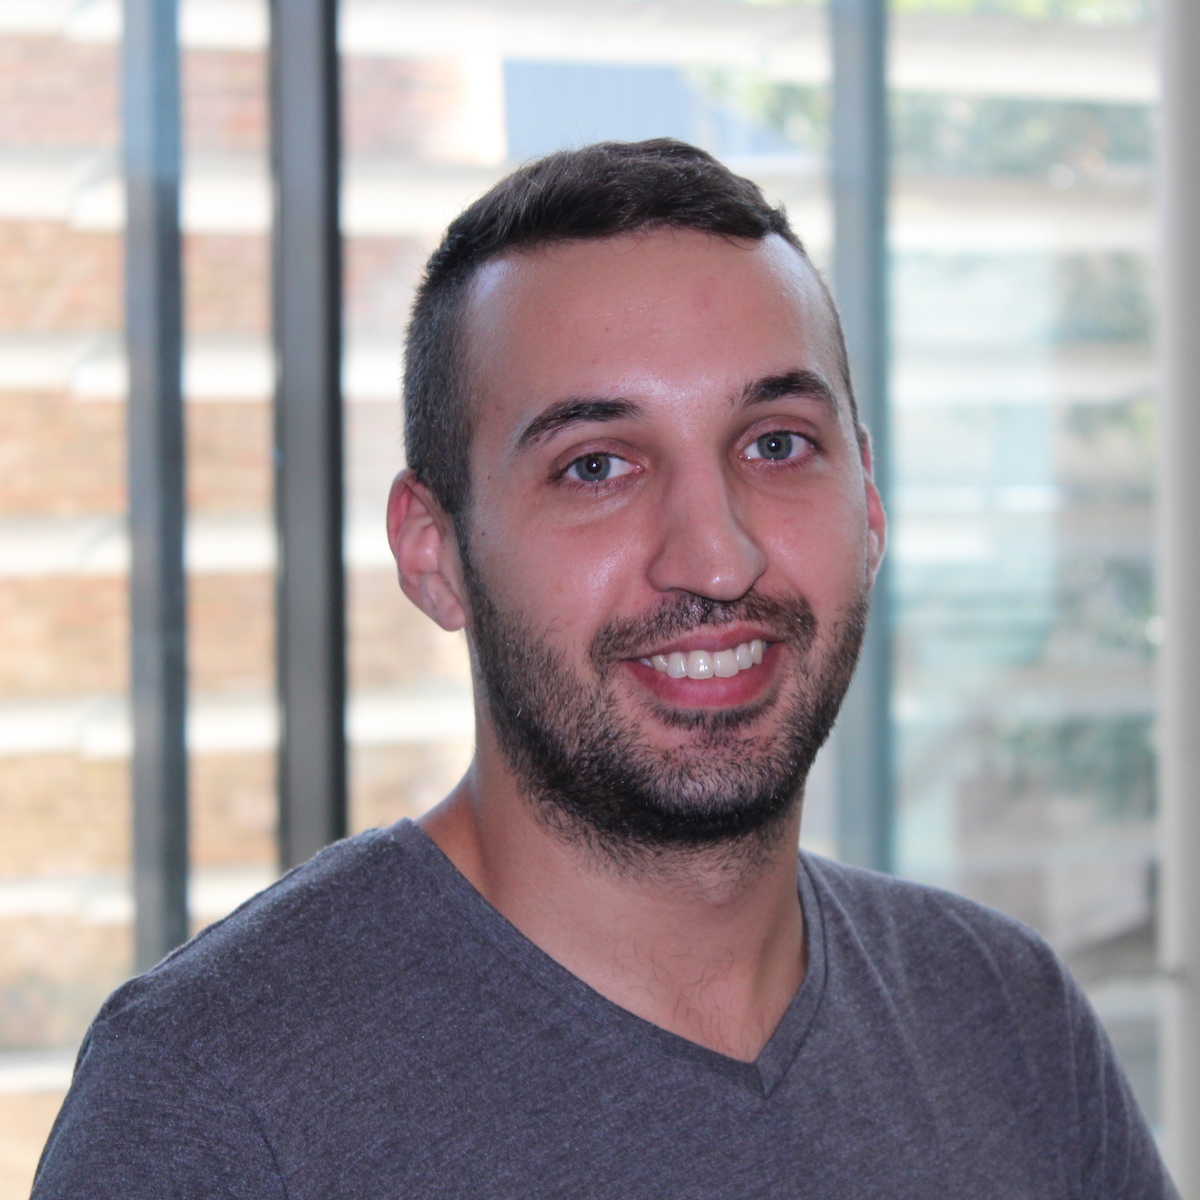
\includegraphics[width=1in,height=1.25in,clip,keepaspectratio]{img/photo_fwilhelmi_1200_1200}}]{Francesc Wilhelmi}
holds a Ph.D. in information and communication technologies (2020), from Universitat Pompeu Fabra (UPF). He is currently working as a postdoctoral researcher in the Mobile Networks department at Centre Tecnològic de Telecomunicacions de Catalunya (CTTC). 
\end{IEEEbiography}

\vspace{-1cm}
% if you will not have a photo at all:
\begin{IEEEbiography}[{
\includegraphics[width=1in,height=1.25in,clip,keepaspectratio]{img/lgiupponi}}]{Lorenza Giupponi} received her Ph.D. degree from UPC, Barcelona, Spain, in 2007. In 2003, she joined the Radio Communications Group, UPC, with a grant of the Spanish Ministry of  Education. From 2006 to 2007, she was an Assistant Professor with UPC. In September 2007, she joined CTTC, where she was a Research Director within the Mobile Networks Department. Between 2007 and 2011 she also was a member of the Executive Committee of CTTC, where she acted as the Director of Institutional Relations. She was a co-recipient of the IEEE CCNC 2010, the IEEE 3rd International Workshop on Indoor and Outdoor Femto Cells 2011, and the IEEE WCNC 2018 Best Paper Award. Between 2015 and 2011, she was a member of the Executive Committee of ns-3 Consortium in charge of coordinating 3GPP related developments. Since 2021 she is a Standardization Researcher in Ericsson.
\end{IEEEbiography}

% insert where needed to balance the two columns on the last page with
% biographies
%\newpage

\vspace{-1cm}
\begin{IEEEbiography}[{
\includegraphics[width=1in,height=1.25in,clip,keepaspectratio]{img/photo_paolo}}]{Paolo Dini} received M.Sc. and Ph.D. from the Universit`a di Roma La Sapienza, in 2001 and 2005, respectively. He is currently a Senior Researcher with the Centre Tecnologic de Telecomunicacions de Catalunya (CTTC). His current research interests include sustainable networking and computing, distributed optimization and optimal control, machine learning, multi-agent systems and data analytics. His research activity is documented in almost 90 peer-reviewed scientific journals and international conference papers. He received two awards from the Cisco Silicon Valley Foundation for his research on heterogeneous mobile networks, in 2008 and 2011, respectively. He has been involved in more than 20 research and development projects. He is currently the Coordinator of CHIST-ERA SONATA project on sustainable computing and communication at the edge and the Scientific Coordinator of the EU H2020 MSCA Greenedge European Training Network on edge intelligence and sustainable computing. He serves as a TPC in many international conferences and workshops and as a reviewer for several scientific journals of the IEEE, Elsevier, ACM, Springer, Wiley.
\end{IEEEbiography}

% You can push biographies down or up by placing
% a \vfill before or after them. The appropriate
% use of \vfill depends on what kind of text is
% on the last page and whether or not the columns
% are being equalized.

%\vfill

% Can be used to pull up biographies so that the bottom of the last one
% is flush with the other column.
%\enlargethispage{-5in}



% that's all folks
\end{document}


